\documentclass[11pt]{article}

\usepackage[a4paper,margin=1in]{geometry}
\usepackage{amsmath,amssymb}
\usepackage{booktabs}
\usepackage{graphicx}
\usepackage{subcaption}
\usepackage[hidelinks]{hyperref}
\usepackage{microtype}
\captionsetup{justification=raggedright,singlelinecheck=false}
\captionsetup[subfigure]{justification=centering,singlelinecheck=true}
\makeatletter
\setlength{\@fptop}{0pt}
\makeatother

\title{DSA5205 Project 1: Machine Learning in Finance}
\author{xxx  \\ A0123456R}
\date{October 2026}

\begin{document}

\maketitle

\begin{abstract}
This report studies model complexity, regularization, and out-of-sample performance in return prediction. Task~1 reproduces the misspecified ridge experiment of Kelly, Malamud, and Zhou (2024); the remaining sections document the extensions, hidden-data predictions, and financial interpretation of neural-network generalization.
\end{abstract}

\section{Task 1: Misspecified Simulation with Ridge}

\subsection{Design and implementation}

Following Kelly, Malamud, and Zhou~\cite{kelly2024}, returns are generated as
\begin{equation}
    R_{t+1}=S_t'\beta^*+\varepsilon_{t+1},
    \qquad S_t\sim\mathcal N(0,I_P),
    \qquad \varepsilon_{t+1}\sim\mathcal N(0,1).
\end{equation}
The vector $\beta^*$ is drawn from an isotropic Gaussian distribution and normalized so that $\|\beta^*\|_2^2=b^*=0.2$. The data-generating complexity is fixed at $c=P/T_{\mathrm{tr}}=10$. In each replication, one random permutation of the $P$ columns is held fixed across the full grid. For a given revealed fraction $q$, only the first $P_1=qP$ permuted columns are observed, so observed complexity is $cq=P_1/T_{\mathrm{tr}}$. This nested observation rule creates misspecification while preserving the sufficiently mixed setting.

The simulation parameters are listed in Table~\ref{tab:task1-parameters} and configured in \path{task1_2/task1.yaml}. Data generation is implemented by \texttt{generate\_data()} in \path{task1_2/generate_data.py}; the experiment loop and nested feature selection are in \path{task1_2/task1.py}.

\begin{table}[htbp]
    \centering
    \caption{Task 1 simulation parameters.}
    \label{tab:task1-parameters}
    \begin{tabular}{ll}
        \toprule
        Parameter & Value \\
        \midrule
        Base seed and replications & $5205$; $50$ \\
        Training and test sizes & $T_{\mathrm{tr}}=500$; $T_{\mathrm{te}}=5000$ \\
        DGP complexity and dimension & $c=10$; $P=5000$ \\
        Signal strength and noise & $b^*=0.2$; $\sigma_\varepsilon=1$ \\
        $cq$ grid & $\{0.50,0.75,0.90,0.95,0.98,1.02,1.05,1.10,$ \\
        & $1.25,1.50,2,3,5,7,10\}$ \\
        Ridge grid & $z\in\{0,0.01,0.1,1,10,50\}$ \\
        \bottomrule
    \end{tabular}
\end{table}

For each observed block, ridge is estimated without an intercept:
\begin{equation}
    \widehat\beta(z)
    =\left(X'X+zT_{\mathrm{tr}}I\right)^{-1}X'y.
\end{equation}
At $z=0$, the implementation uses the Moore--Penrose pseudoinverse. For $z>0$, it solves the primal system when $P_1\leq T_{\mathrm{tr}}$ and the equivalent dual system otherwise; see \texttt{fit\_ridge()} in \path{task1_2/fit_ridge.py}.

All quantities are evaluated on the independent test set. With $\widehat R_{t+1}=S_t'\widehat\beta$ and timing return $R^\pi_{t+1}=\widehat R_{t+1}R_{t+1}$, the reported metrics are
\begin{align}
R^2_{\mathrm{paper}}
    &=1-\frac{\mathbb E[(R_{t+1}-\widehat R_{t+1})^2]}
                 {\mathbb E[R_{t+1}^2]}, \\
\mathbb E[R^\pi_{t+1}]
    &=\mathbb E[\widehat R_{t+1}R_{t+1}], \\
\mathrm{SR}
    &=\frac{\mathbb E[R^\pi_{t+1}]}
            {\sqrt{\mathbb E[(R^\pi_{t+1})^2]}},
\qquad
\|\widehat\beta(z)\|_2.
\end{align}
Their sample analogues are computed by \texttt{calculate\_metrics()} in \path{task1_2/test_metrics.py}.

\subsection{Results}

Figure~\ref{fig:task1-results} reports averages over the 50 replications. It is the finite-sample analogue of Figures 4--6 in Kelly, Malamud, and Zhou~\cite{kelly2024}, which plot population limits rather than simulated estimates. The ridgeless specification displays the expected instability around the interpolation threshold $cq=1$: $R^2_{\mathrm{paper}}$ falls to about $-50$ at $cq=0.98$--$1.02$, while $\|\widehat\beta\|_2$ rises above $7.5$. These extremes, and timing returns above $0.02$, are clipped by the displayed axes. As in the paper's Figure 4, both effects abate for $cq>1$ because overparameterized minimum-norm regression supplies implicit regularization. Explicit shrinkage smooths the interpolation singularity; $z=10$ or $50$ keeps $R^2_{\mathrm{paper}}$ close to zero and the coefficient norm small.

The expected-return panel has the same broad message as the left panel of the paper's Figure 5: very simple models have low timing returns because they observe too little of the DGP, and additional features improve approximation. In the population benchmark, ridgeless expected return rises to $b^*/c=0.02$ at $cq=1$ and is exactly flat thereafter. The simulation approaches roughly $0.018$--$0.019$ away from interpolation, but overshoots and fluctuates near $cq=1$; for example, its ridgeless mean is $0.0347$ at $cq=1.02$. This difference is consistent with finite training and test samples and the nonlinear effect of near-singular estimates, rather than a contradiction of the limiting result. The paper's Figure 5 also reports portfolio volatility; the project instead requires the Sharpe ratio and coefficient norm, which expose the same interpolation instability through risk adjustment and parameter dilation.

The Sharpe panel closely reproduces the paper's Figure 6. Ridgeless and lightly regularized curves show ``double ascent'': Sharpe rises at low complexity, dips near interpolation as coefficient and portfolio risk explode, and rises again for $cq>1$. Nontrivial shrinkage removes most of this dip, producing an approximately permanent ascent. At $cq=10$, all curves converge to about $0.049$--$0.050$; the largest value on the simulated grid is $0.0505$ for $z=50$. For $\Psi=I$, the paper's optimal shrinkage is
\begin{equation}
    z^*(q)=\frac{c\{1+b^*(1-q)\}}{b^*}=60-10q,
\end{equation}
so $z=50$ is exactly optimal at $q=1$ and is close to the theoretical range over the grid. Theorem 1's monotone, concave improvement applies to this optimally adjusted $z^*(q)$, not to every fixed-$z$ curve. Overall, the finite-sample experiment supports the virtue-of-complexity mechanism: under misspecification and sufficient mixing, observing more signals improves risk-adjusted timing performance even when conventional out-of-sample $R^2$ remains negative.

\begin{figure}[htbp]
    \centering
    \begin{subfigure}[t]{0.49\textwidth}
        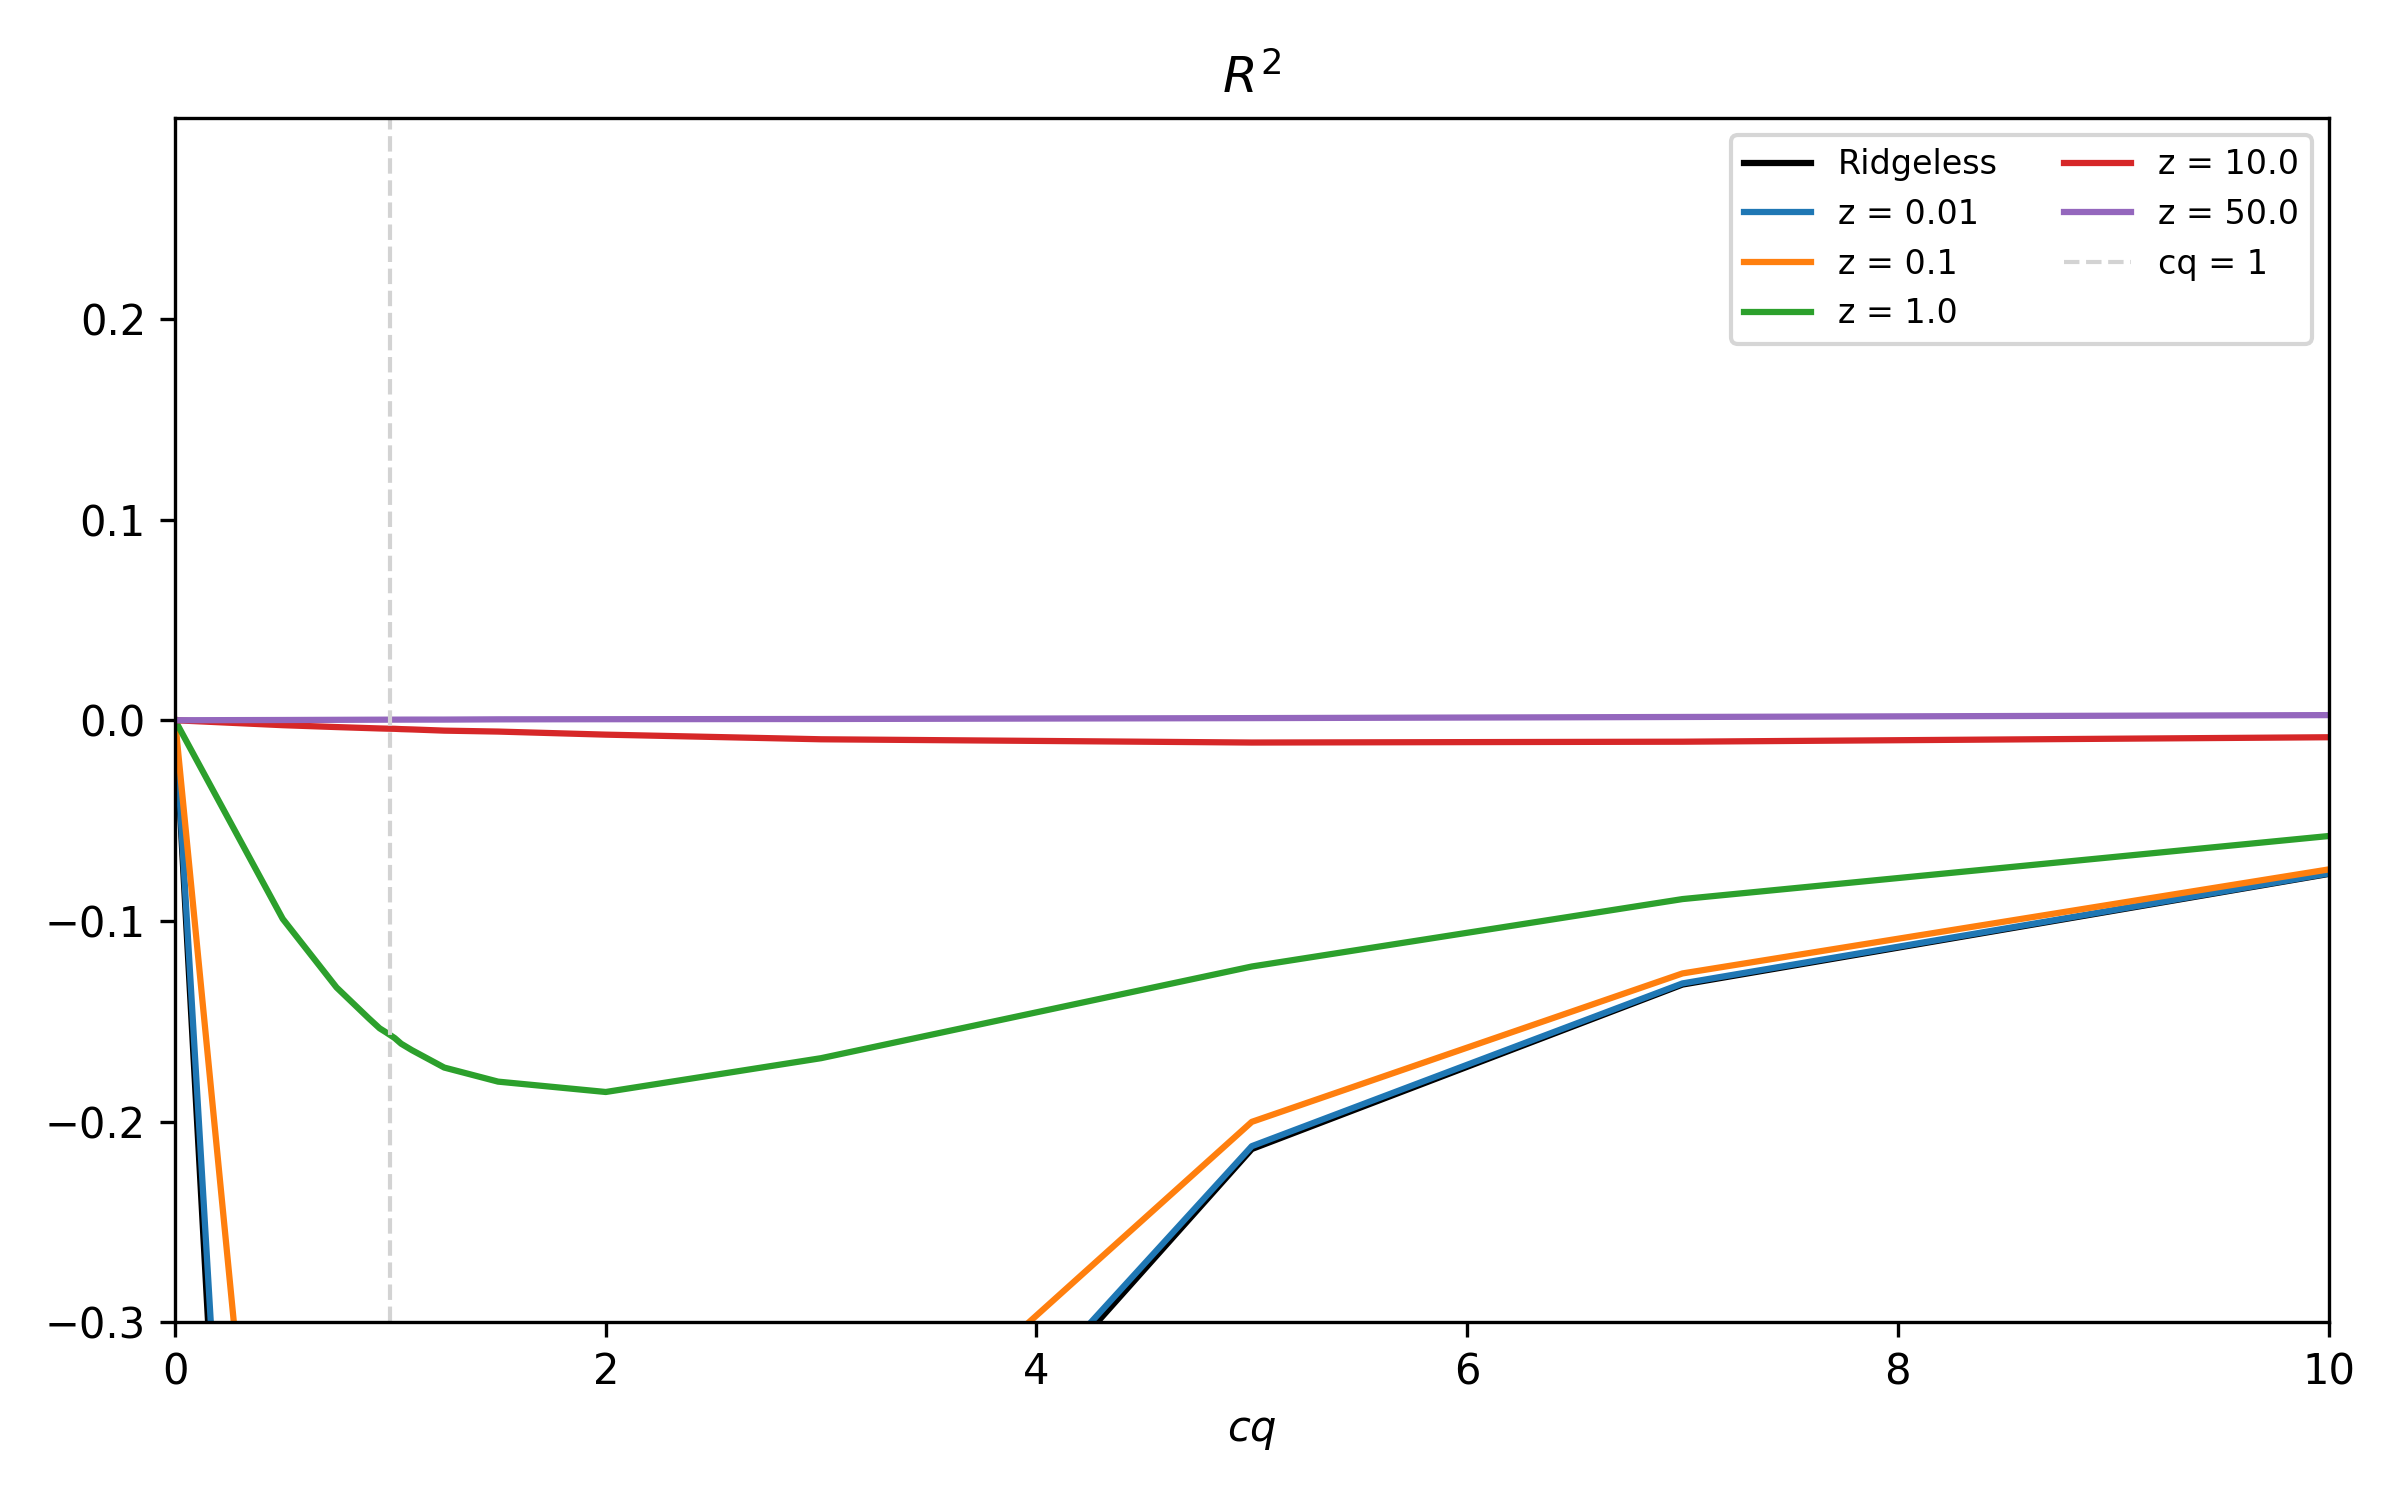
\includegraphics[width=\linewidth]{task1_2/task1_result_20261007_202024/r2_paper_vs_cq.png}
        \caption{$R^2_{\mathrm{paper}}$.}
    \end{subfigure}
    \hfill
    \begin{subfigure}[t]{0.49\textwidth}
        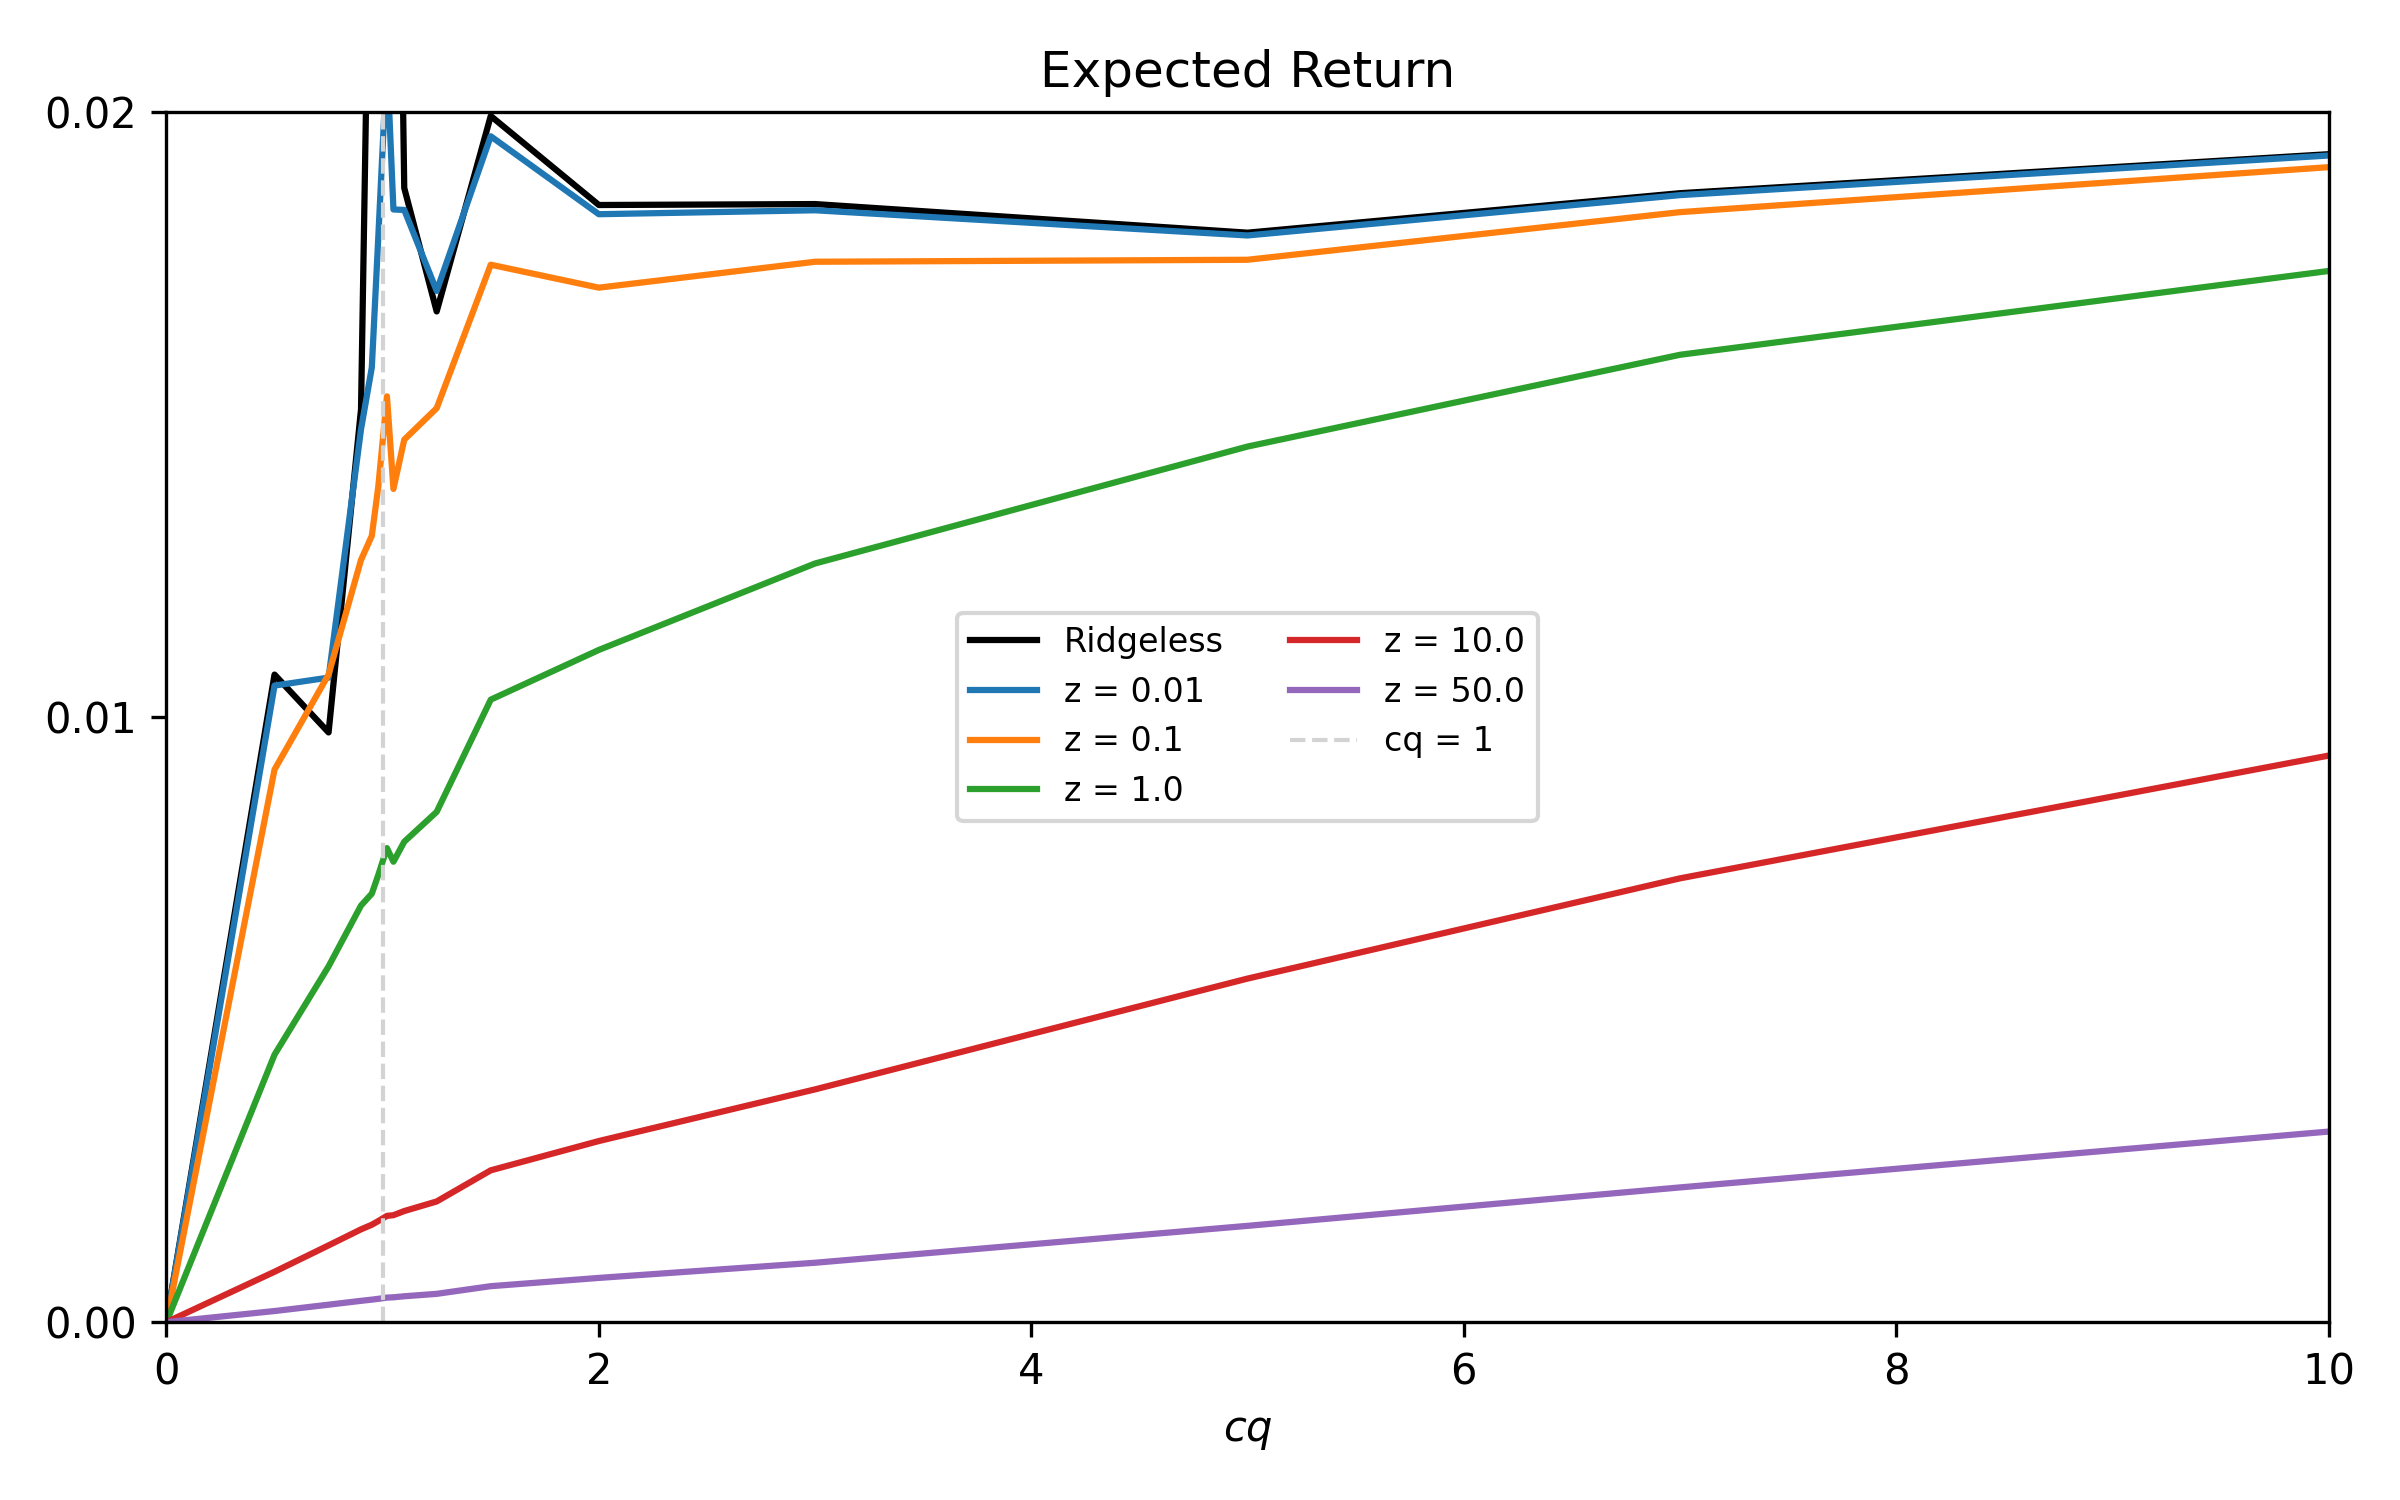
\includegraphics[width=\linewidth]{task1_2/task1_result_20261007_202024/expected_timing_return_vs_cq.png}
        \caption{Expected timing return.}
    \end{subfigure}

    \begin{subfigure}[t]{0.49\textwidth}
        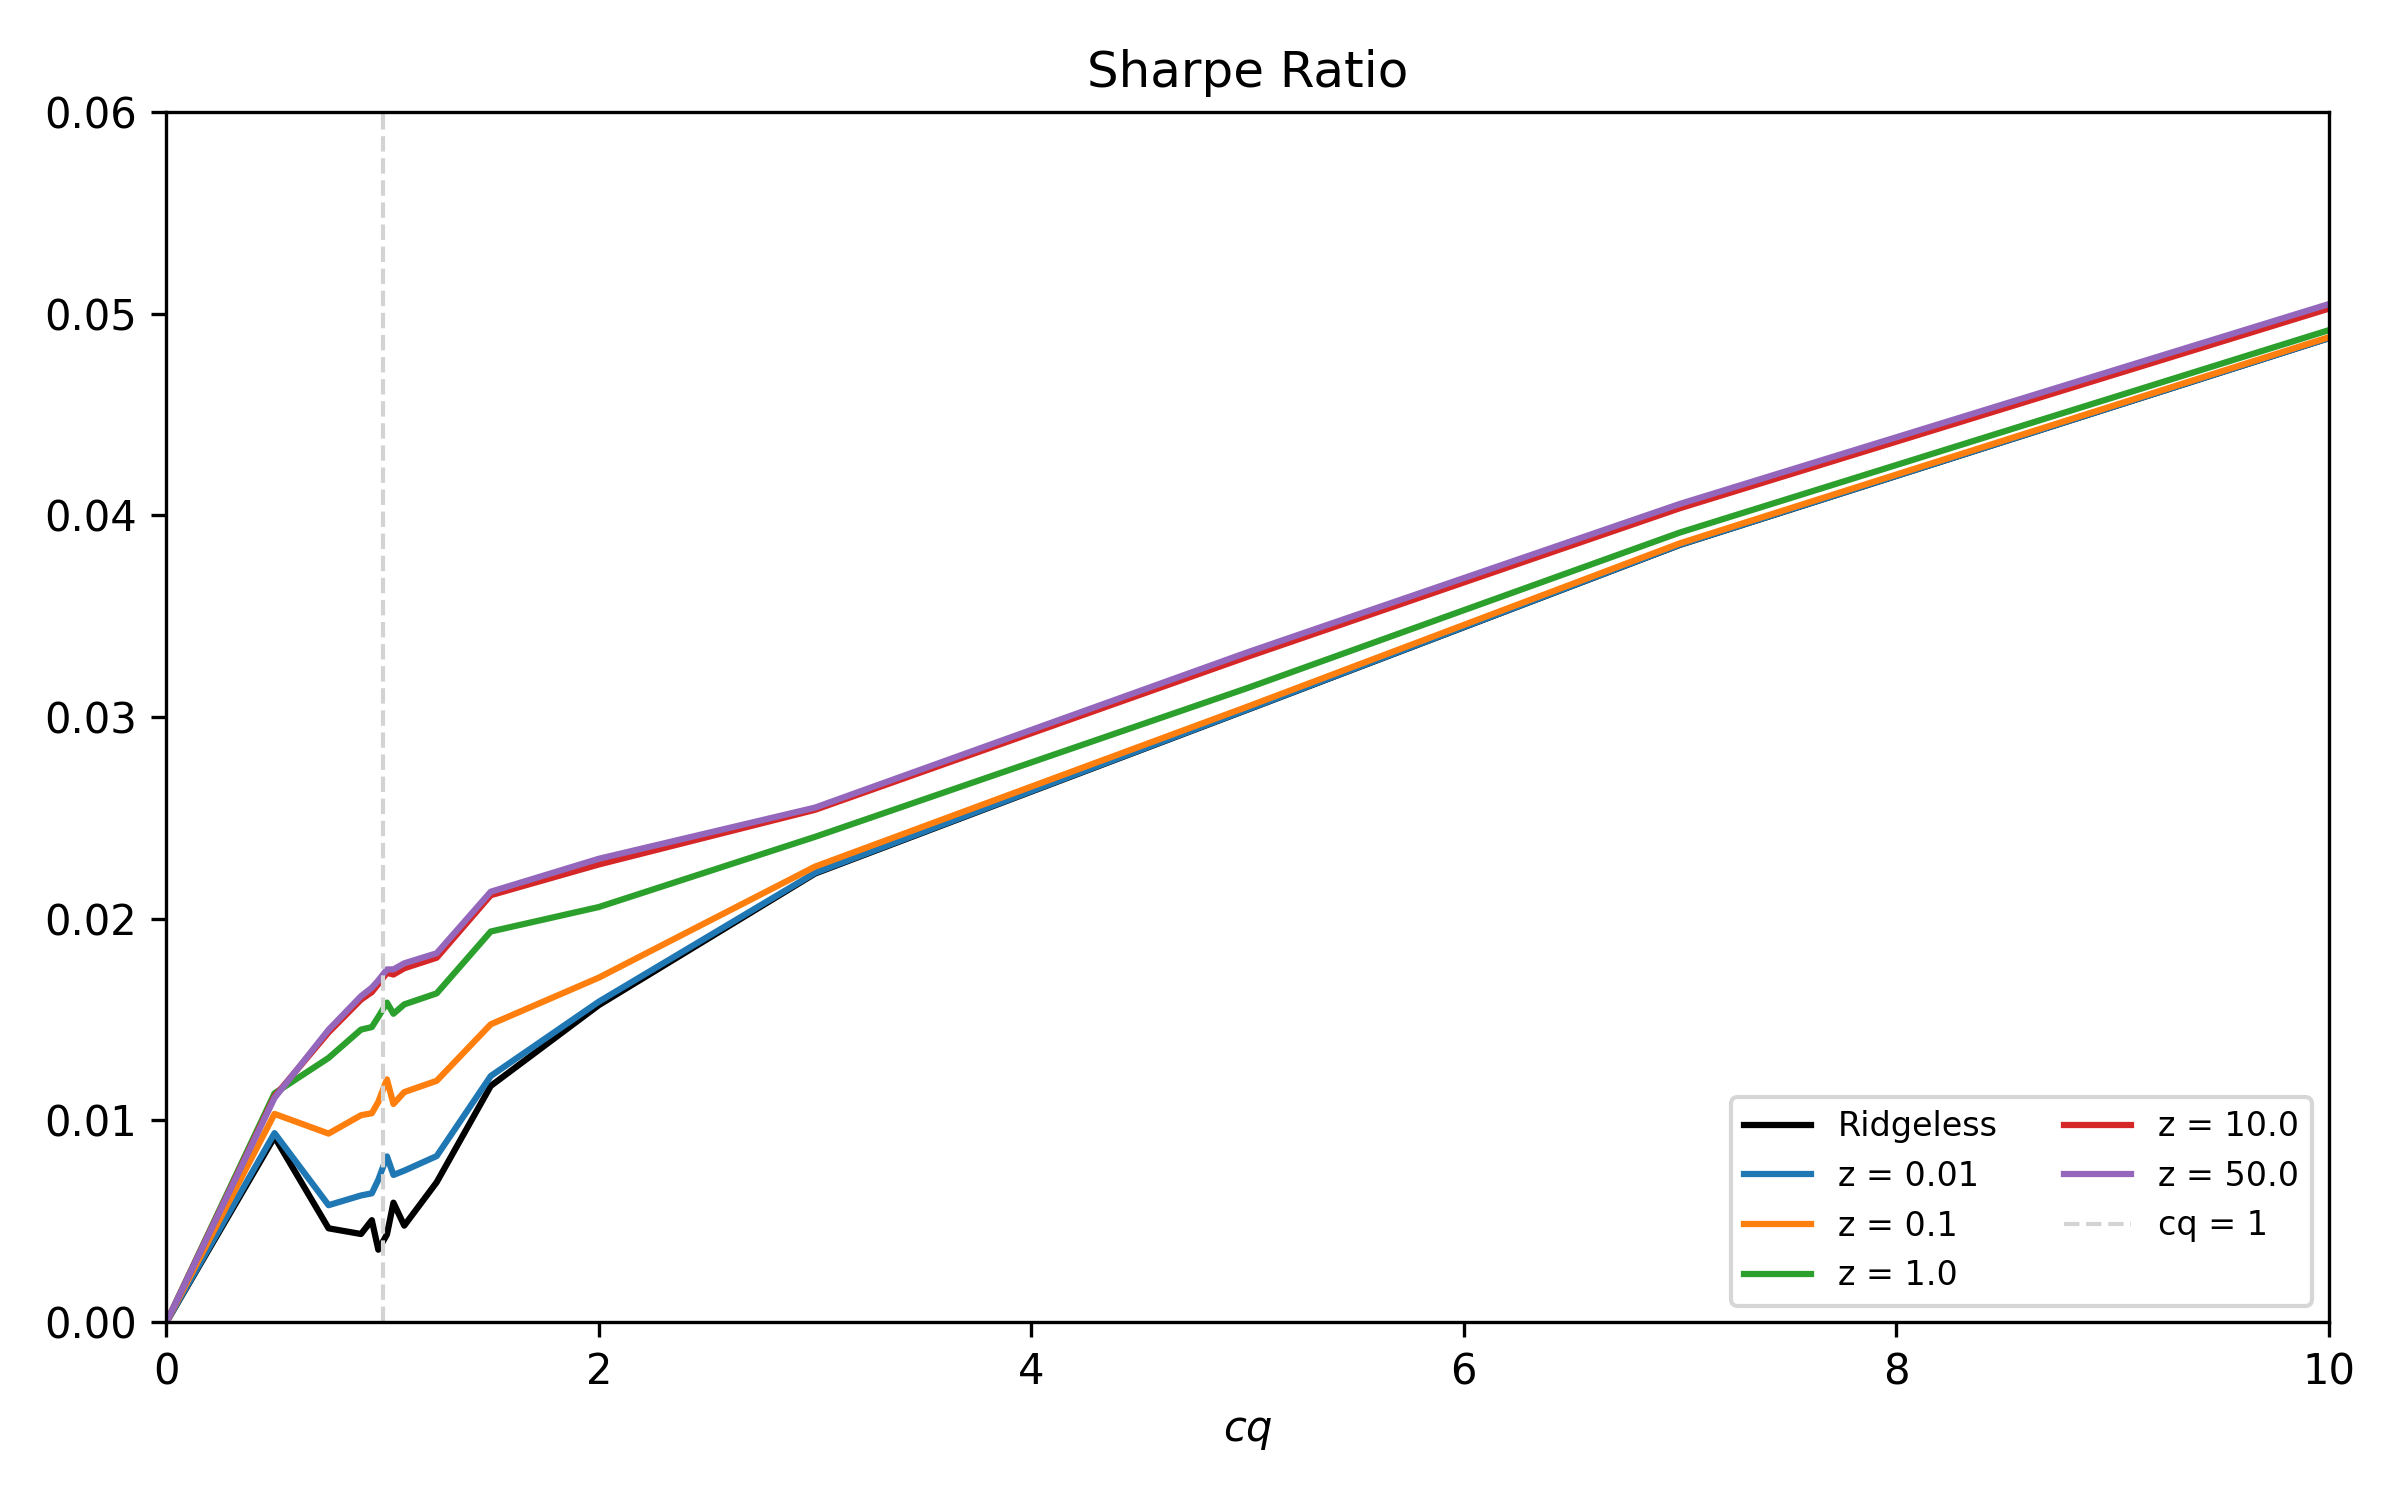
\includegraphics[width=\linewidth]{task1_2/task1_result_20261007_202024/sharpe_paper_vs_cq.png}
        \caption{Paper Sharpe ratio.}
    \end{subfigure}
    \hfill
    \begin{subfigure}[t]{0.49\textwidth}
        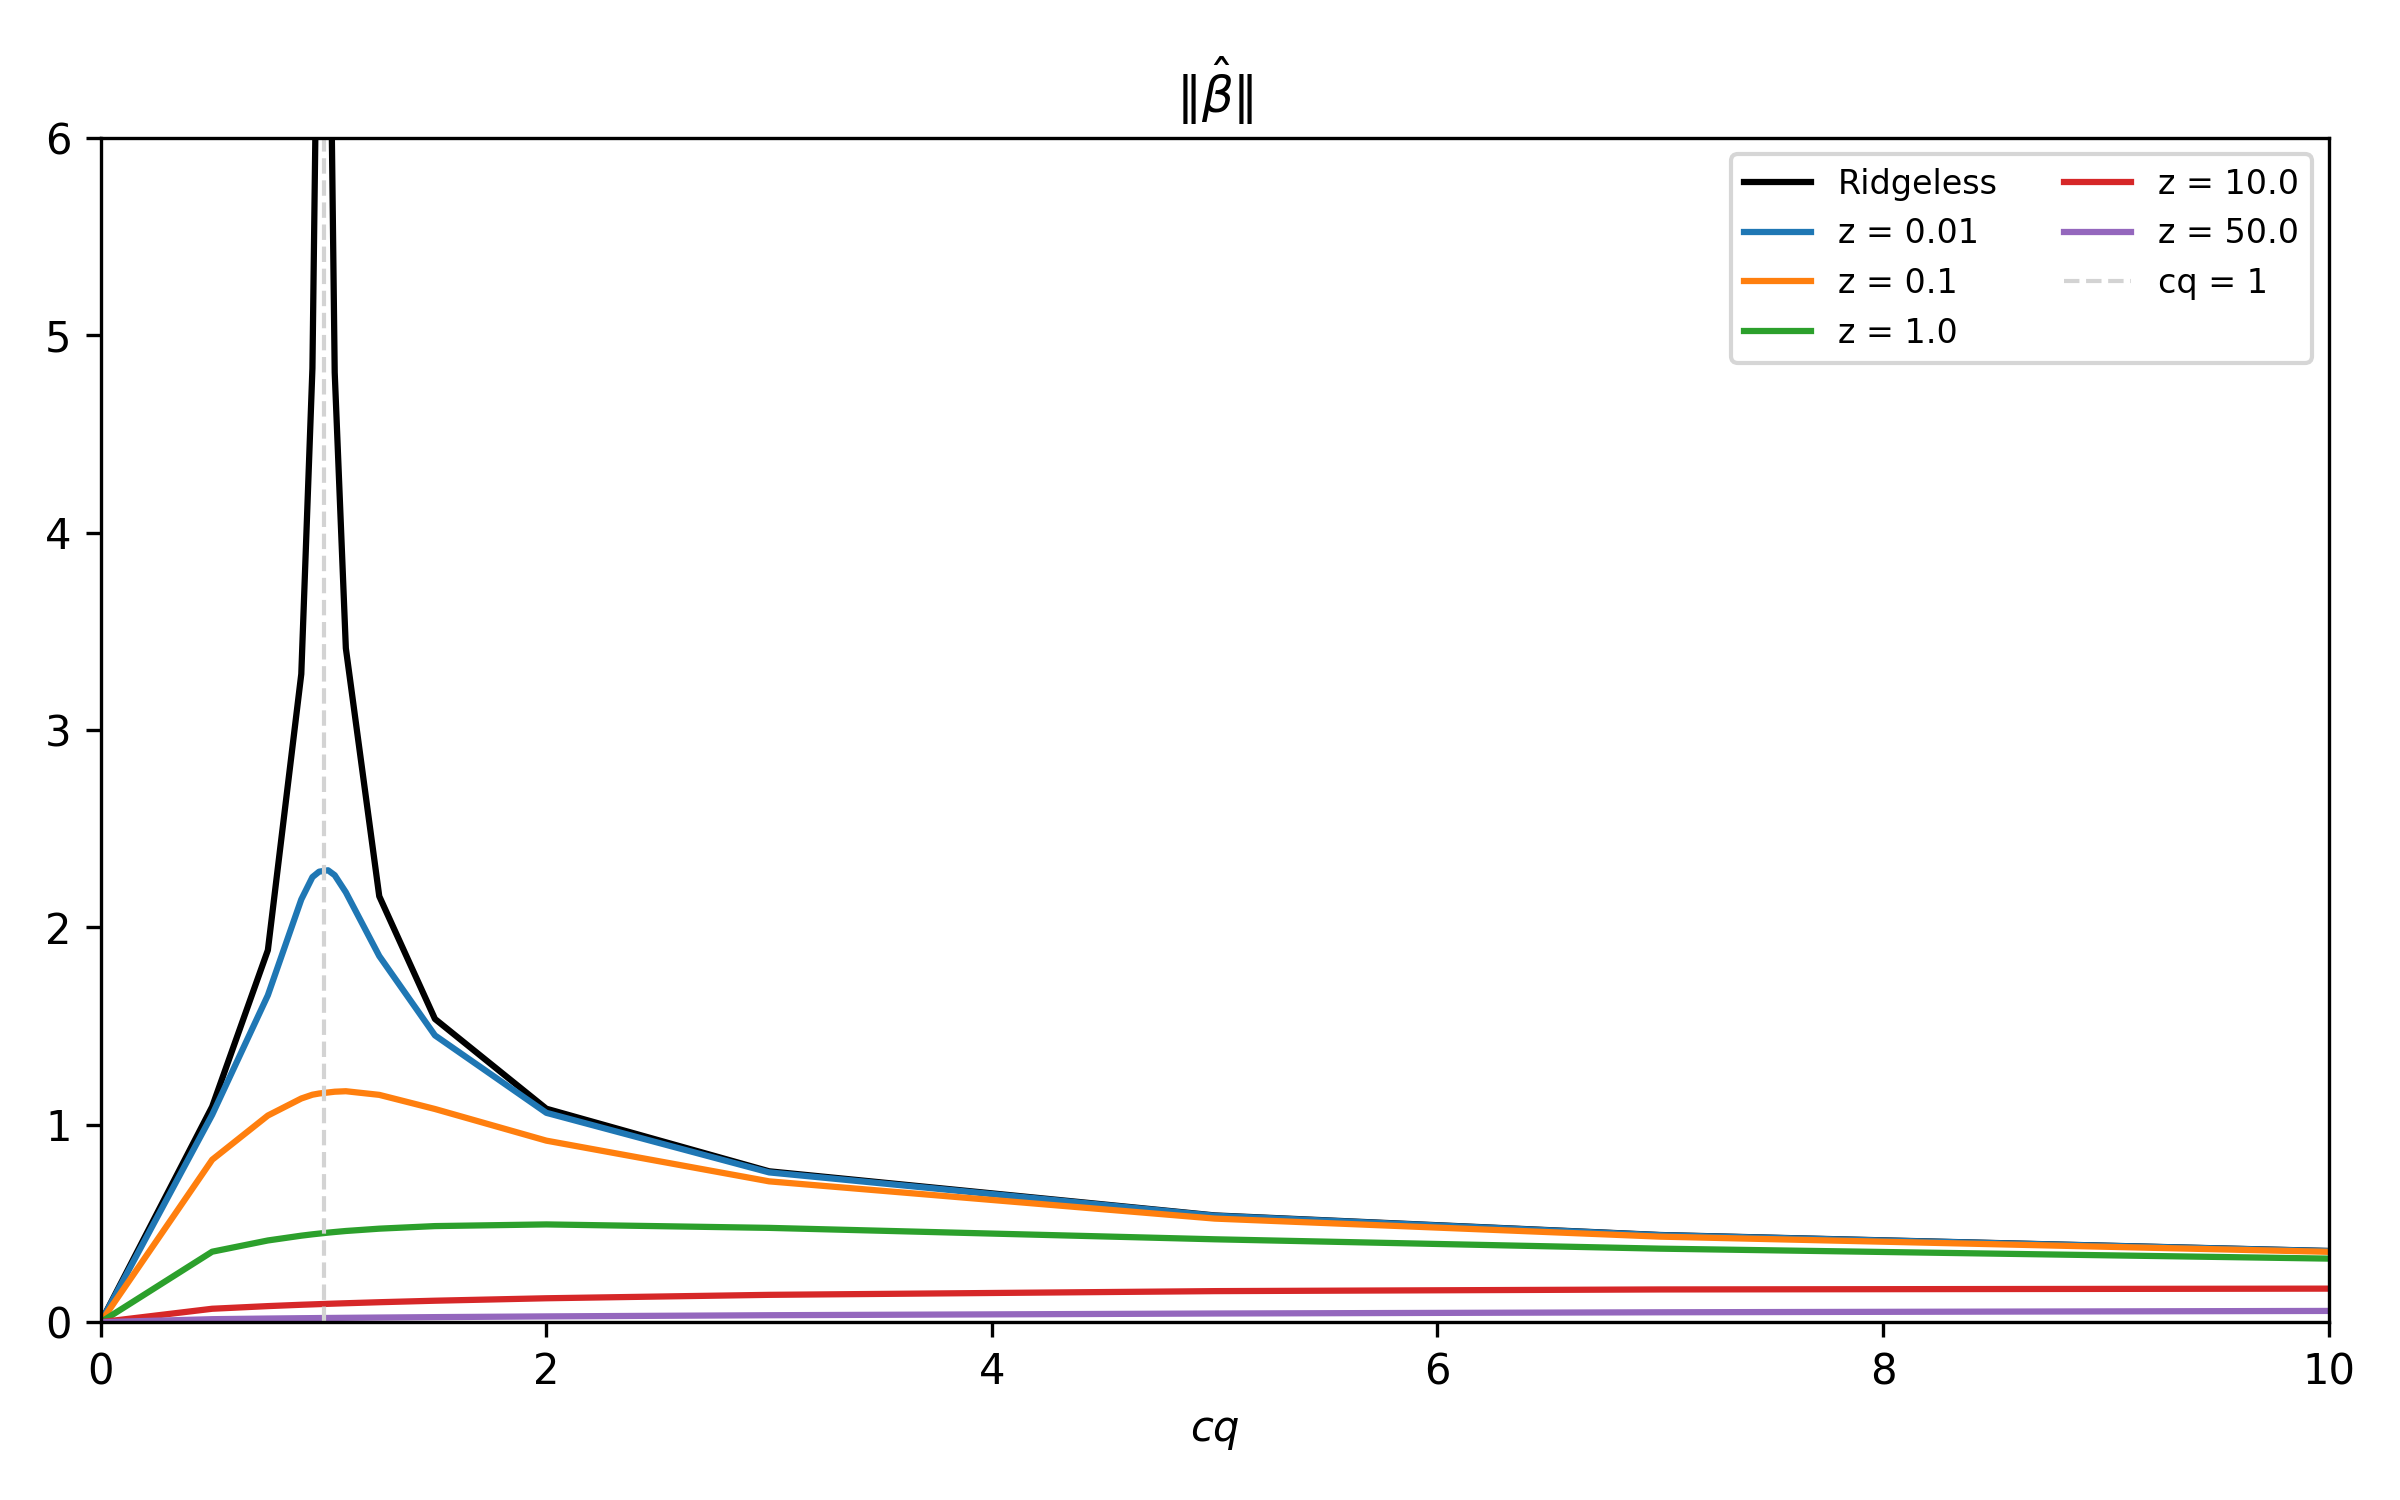
\includegraphics[width=\linewidth]{task1_2/task1_result_20261007_202024/beta_norm_vs_cq.png}
        \caption{Coefficient norm.}
    \end{subfigure}
    \caption{Finite-sample counterparts of Figures 4--6 in Kelly, Malamud, and Zhou~\cite{kelly2024}, averaged over 50 replications. The dashed line marks $cq=1$; displayed axes clip the interpolation extremes. All four panels are produced by \texttt{plot\_results()} in \texttt{task1\_2/plot\_results.py} from \texttt{results.csv}.}
    \label{fig:task1-results}
\end{figure}

\section{Task 2: Alternative Model}

\subsection{Method and experimental control}
Task~2 is implemented in \path{task1_2/task2.py} and reads the shared
configuration in \path{task1_2/task2.yaml}. For every replication it
reuses the Task~1 seed, data-generating process, train/test split, fixed feature
permutation, and $cq$ grid, replacing ridge regression with Lasso regression.
The estimator solves
\begin{equation}
    \widehat\beta(\alpha)
    =\arg\min_{\beta}\left\{
      \frac{1}{2T_{\mathrm{tr}}}\|y-X\beta\|_2^2
      +\alpha\|\beta\|_1
    \right\},
\end{equation}
without an intercept. The fixed grid is
$\alpha\in\{0.001,0.003,0.01,0.03,0.1\}$. The complete path is fitted by
\texttt{lasso\_path()} with warm starts, random coordinate selection, at most
$3000$ iterations, and tolerance $10^{-3}$. The same out-of-sample metrics are
then computed by \texttt{calculate\_metrics()} in
\path{task1_2/test_metrics.py}. Thus differences from Task~1 reflect the
estimator rather than different simulated samples.

\subsection{Results and comparison with ridge}
Figure~\ref{fig:task2-results} shows the averages over 50 replications. Weak
penalties ($\alpha=0.001$ and $0.003$) retain an interpolation effect: near
$cq=1$, coefficient norms peak at approximately $2.54$ and $1.71$, and
$R^2_{\mathrm{paper}}$ reaches about $-5.36$ and $-2.41$, respectively. This
is substantially less extreme than ridgeless regression in Task~1, whose norm
exceeds $7.5$ and whose $R^2_{\mathrm{paper}}$ falls below $-50$, although it
does not eliminate instability. Increasing $\alpha$ shrinks the norm and
smooths the threshold. At $\alpha=0.1$, $R^2_{\mathrm{paper}}$ remains near
zero, but both expected return and Sharpe are small because the model is
strongly underfit.

The economic metrics expose the bias--variance trade-off. The smallest
penalty attains the largest expected timing return, $0.0211$ at $cq=1.02$,
but its simultaneous prediction error keeps Sharpe at only $0.0075$ there.
For $cq>1$, the weakly penalized Sharpe curves recover and reach about
$0.0224$ at $cq=10$. Moderate $\alpha=0.03$ gives the best Sharpe around the
interpolation region and a relatively smooth curve, but it plateaus near
$0.0197$. Strong $\alpha=0.1$ suppresses both signal and risk and reaches only
$0.0129$ at $cq=10$.

Lasso therefore reproduces the broad virtue-of-complexity pattern---timing
performance generally improves as more signals are revealed---but it
underperforms the best ridge specification on this dense Gaussian DGP. At
$cq=10$, the best Lasso Sharpe on the grid is $0.0224$, compared with $0.0505$
for ridge with $z=50$; its corresponding $R^2_{\mathrm{paper}}$ is $-0.390$,
compared with $0.0026$ for ridge. This gap is consistent with model mismatch:
the $\ell_1$ penalty is designed to exploit sparsity, whereas the true
$\beta^*$ spreads a small signal across all $P$ coordinates. Lasso discards
many individually weak but collectively useful predictors, while the
$\ell_2$ penalty retains and stabilizes them.

\begin{figure}[htbp]
    \centering
    \begin{subfigure}[t]{0.49\textwidth}
        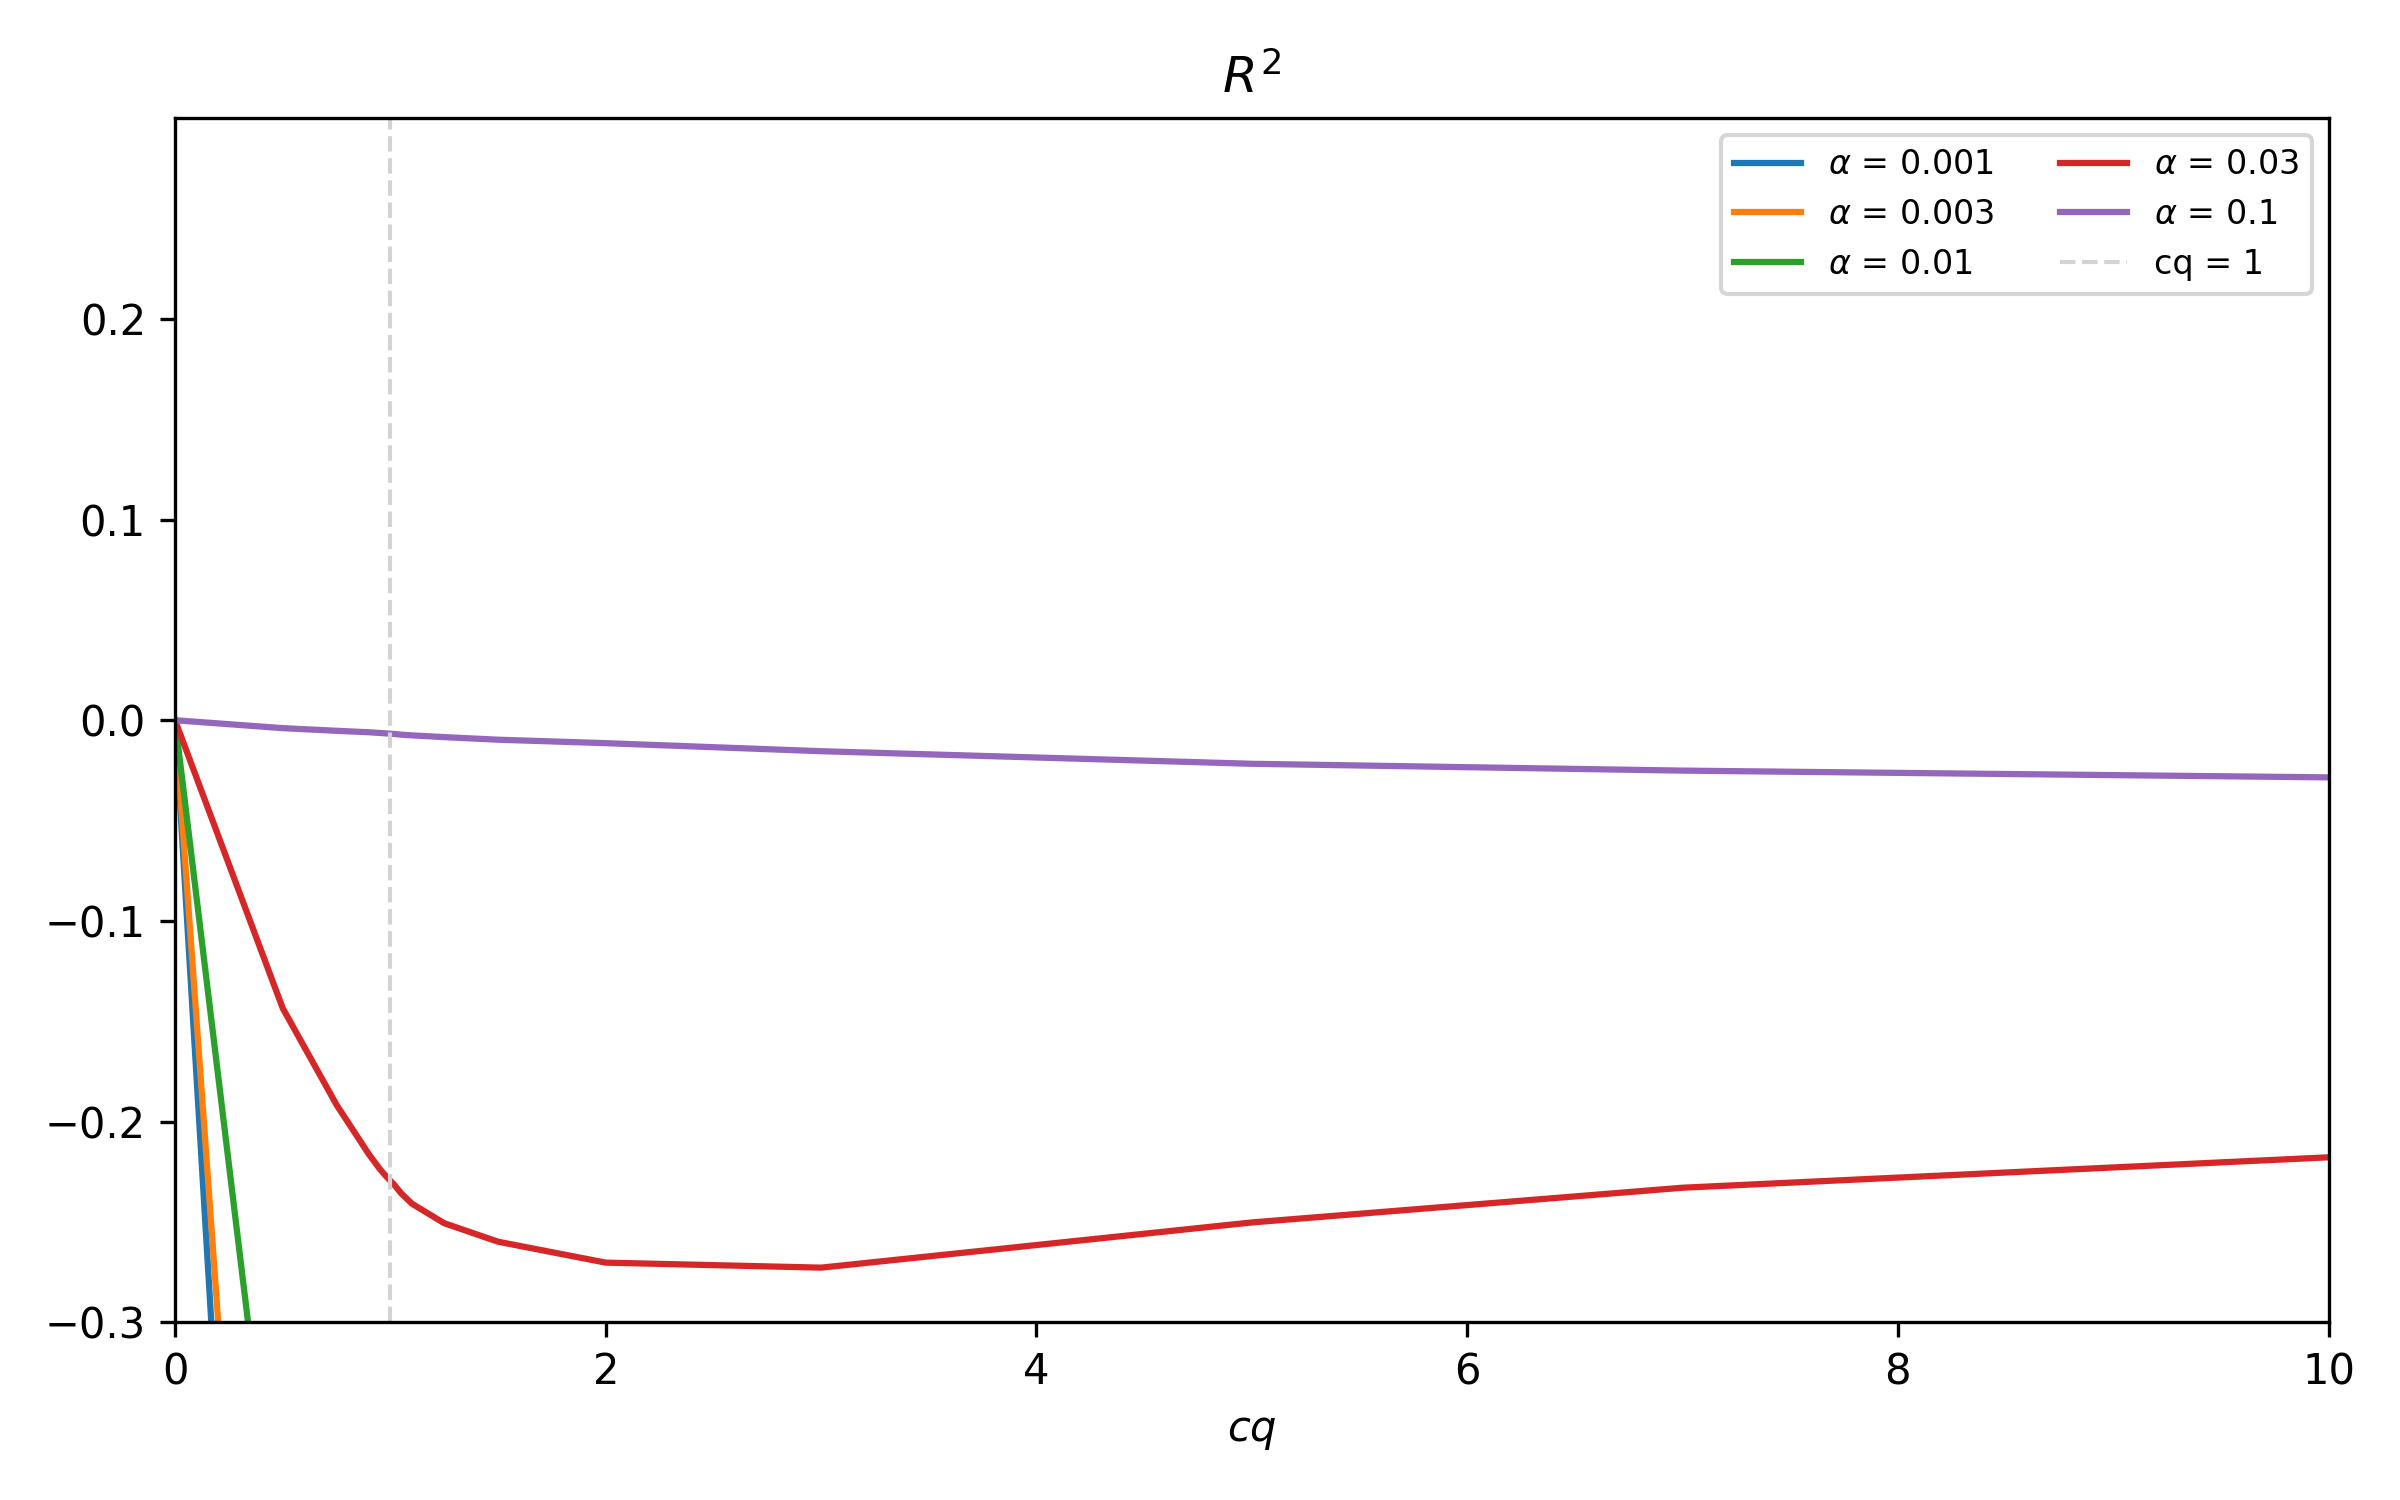
\includegraphics[width=\linewidth]{task1_2/task2_result_20261008_205656/r2_paper_vs_cq.png}
        \caption{$R^2_{\mathrm{paper}}$.}
    \end{subfigure}
    \hfill
    \begin{subfigure}[t]{0.49\textwidth}
        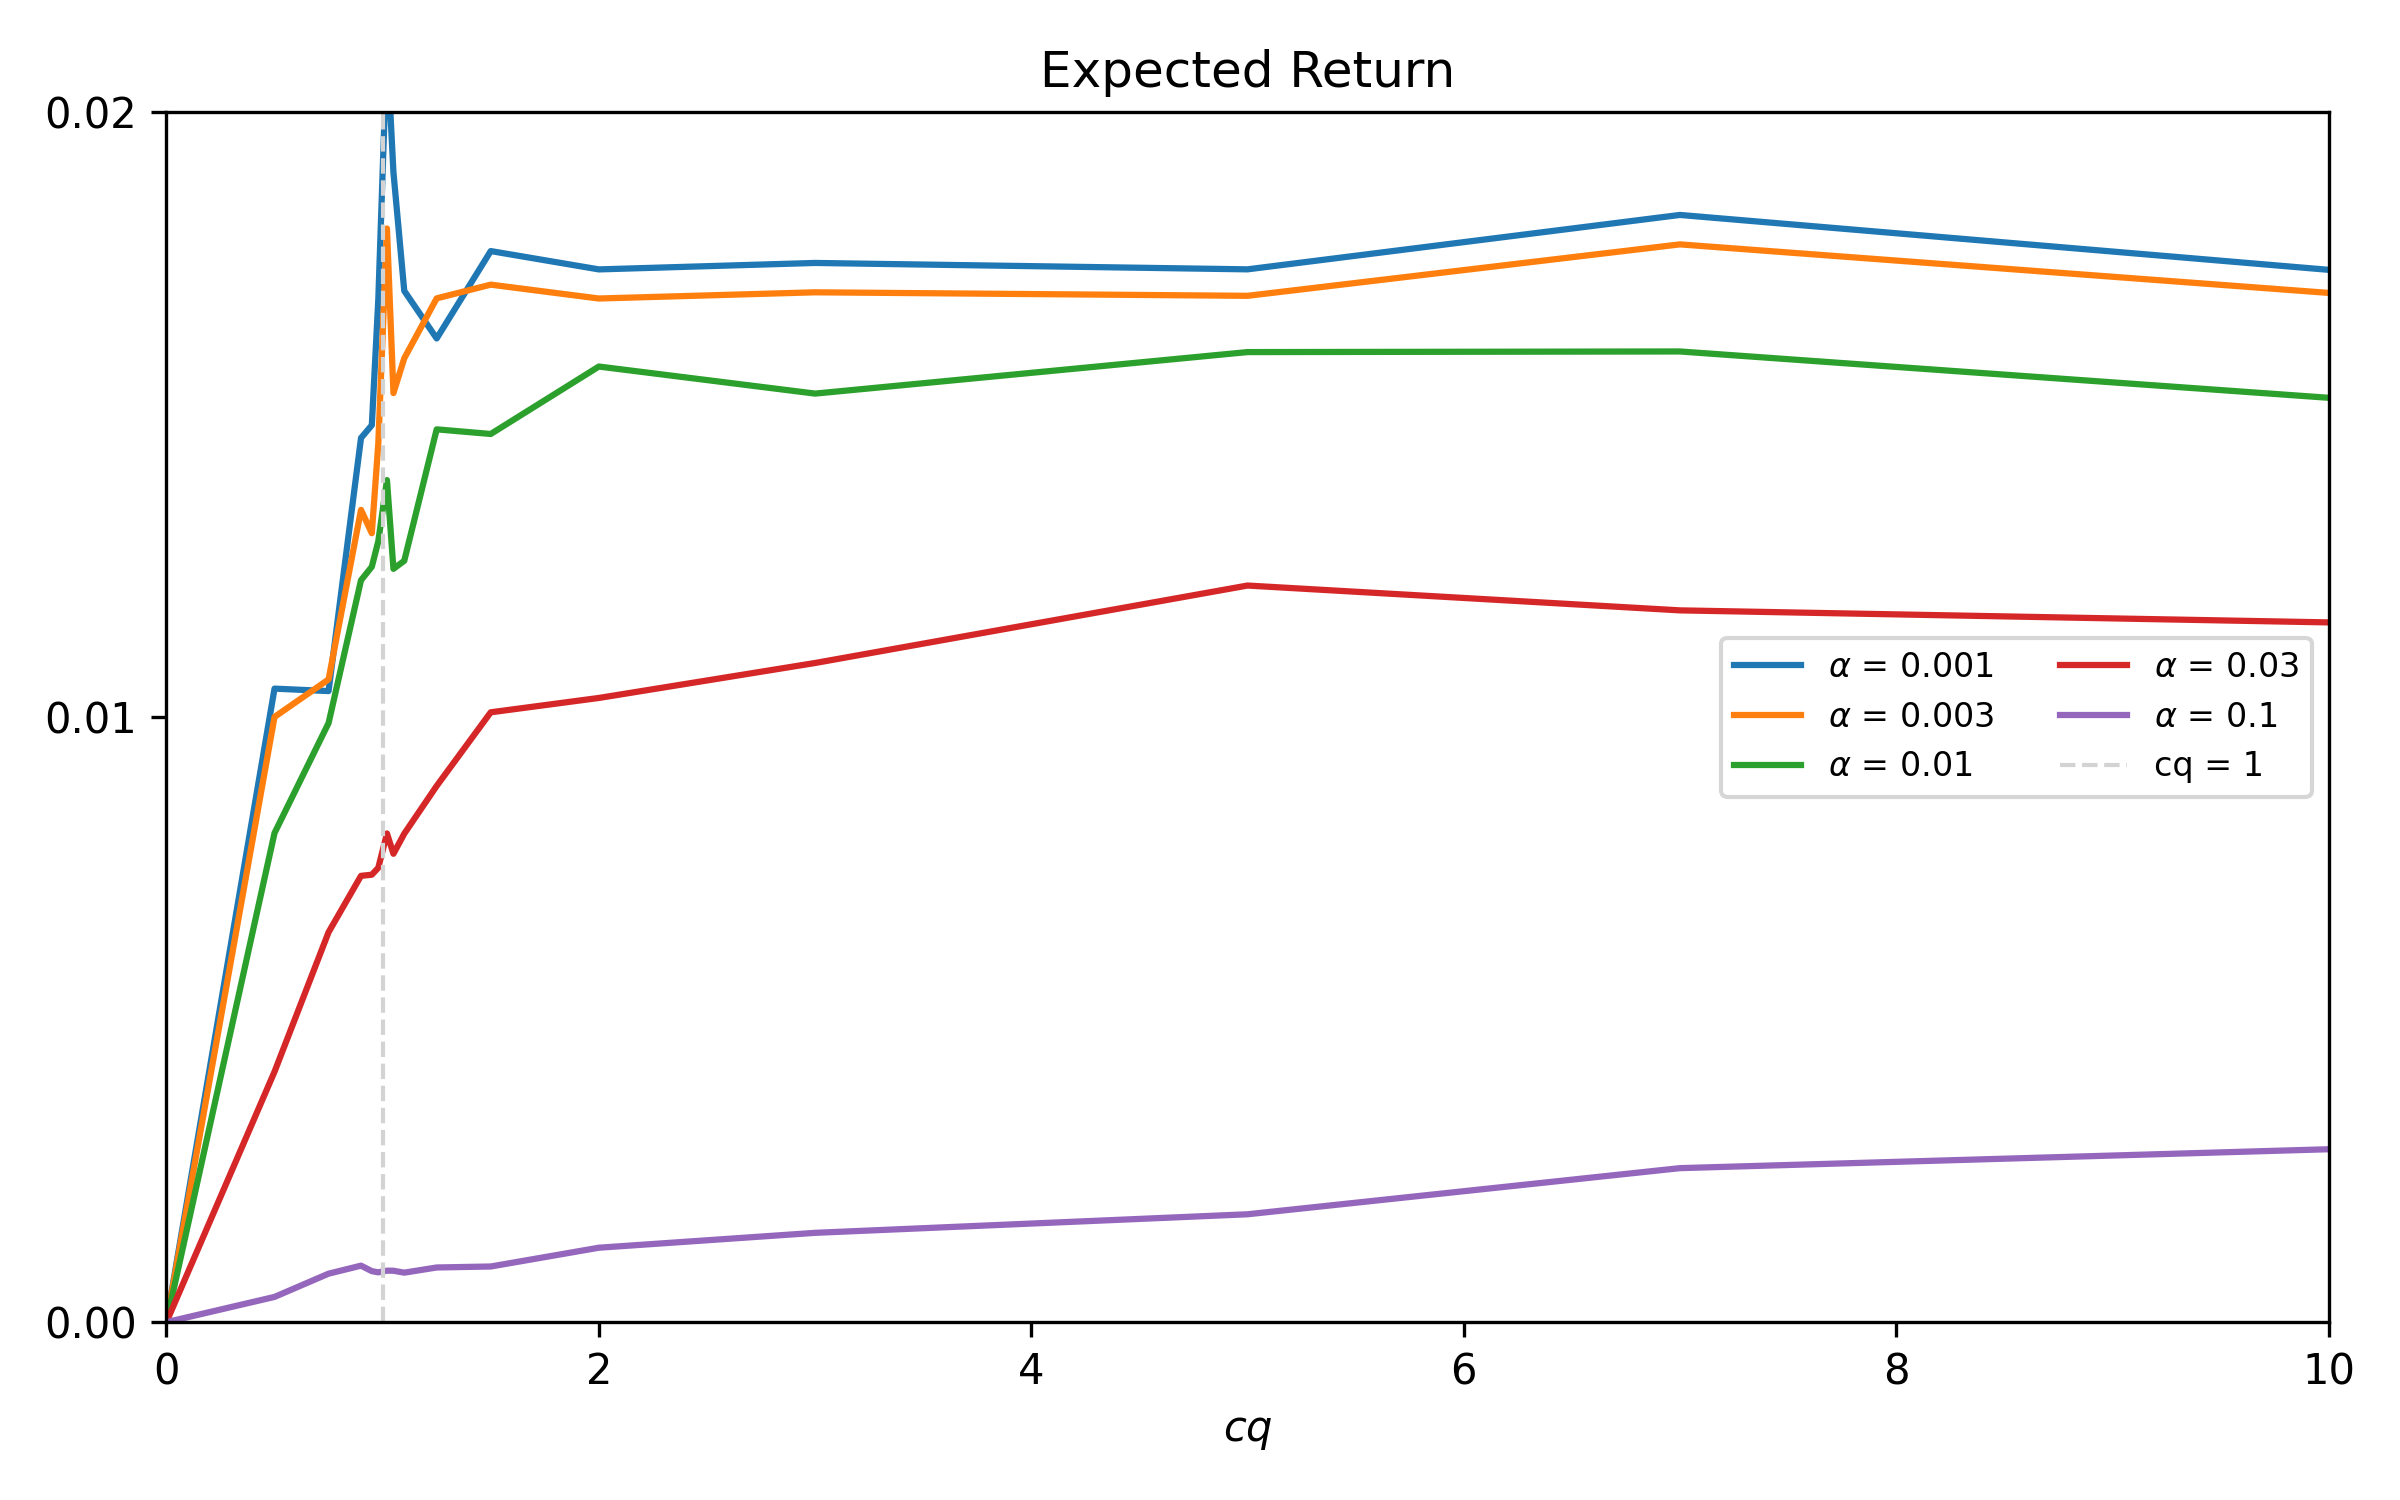
\includegraphics[width=\linewidth]{task1_2/task2_result_20261008_205656/expected_timing_return_vs_cq.png}
        \caption{Expected timing return.}
    \end{subfigure}

    \begin{subfigure}[t]{0.49\textwidth}
        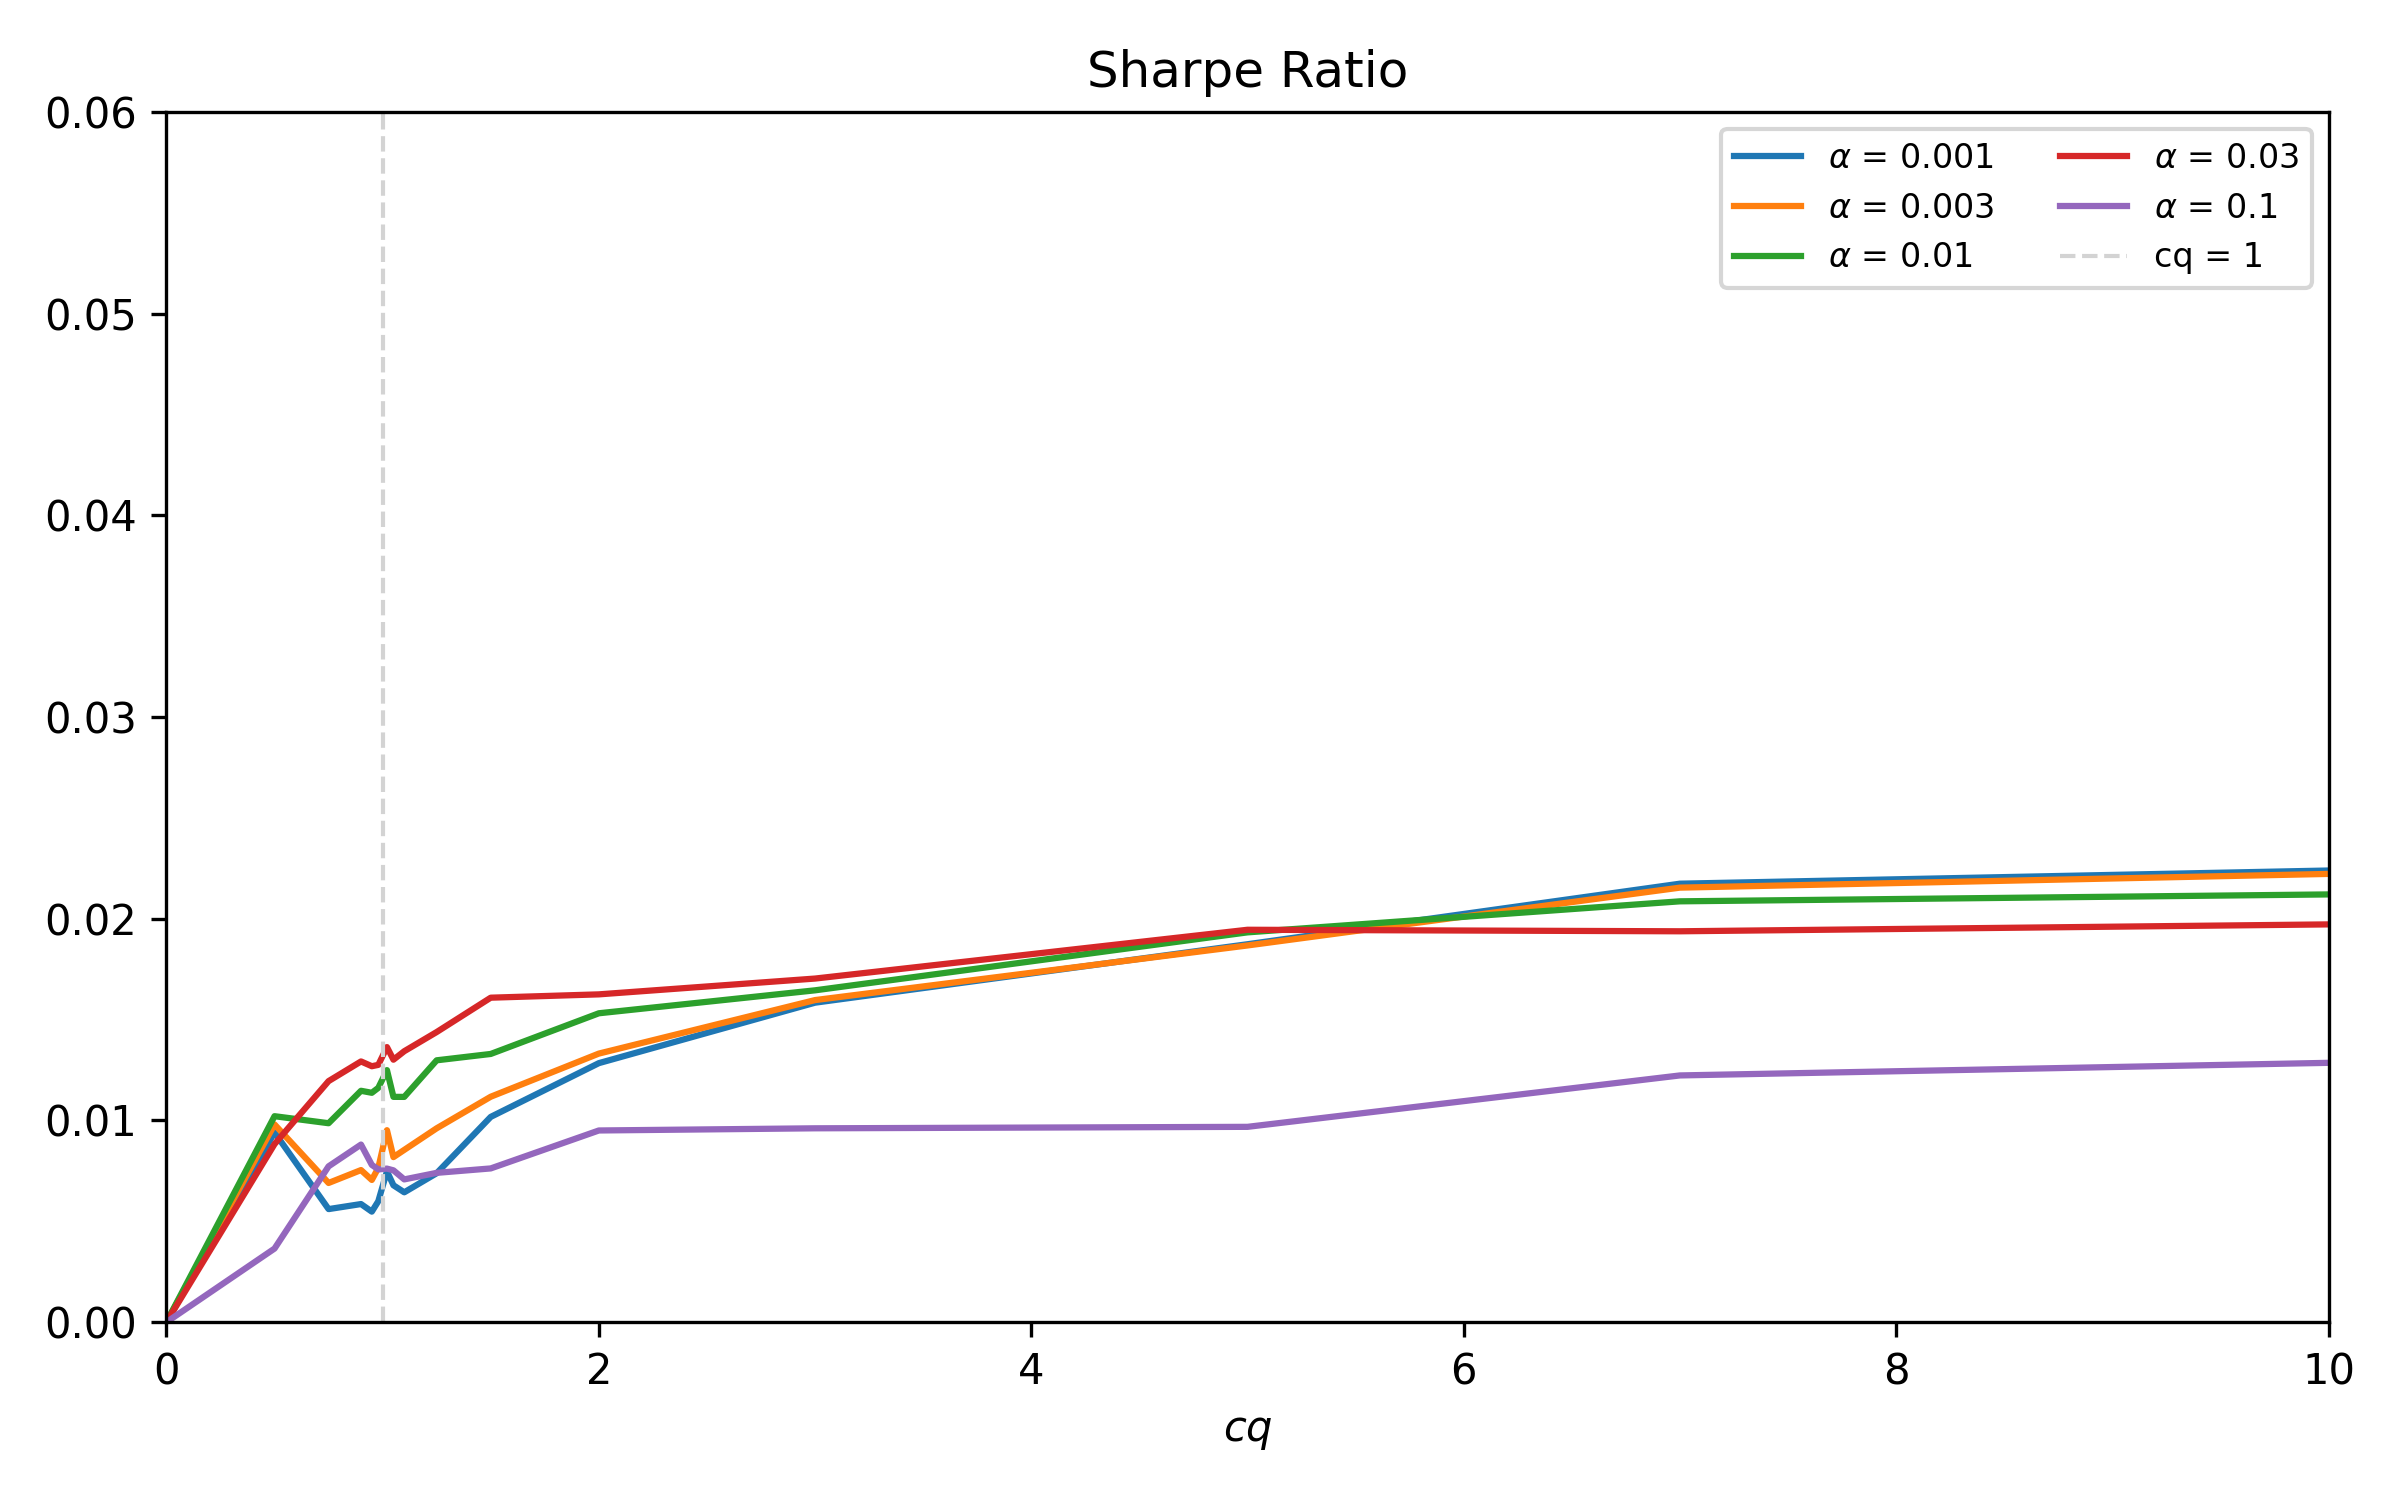
\includegraphics[width=\linewidth]{task1_2/task2_result_20261008_205656/sharpe_paper_vs_cq.png}
        \caption{Paper Sharpe ratio.}
    \end{subfigure}
    \hfill
    \begin{subfigure}[t]{0.49\textwidth}
        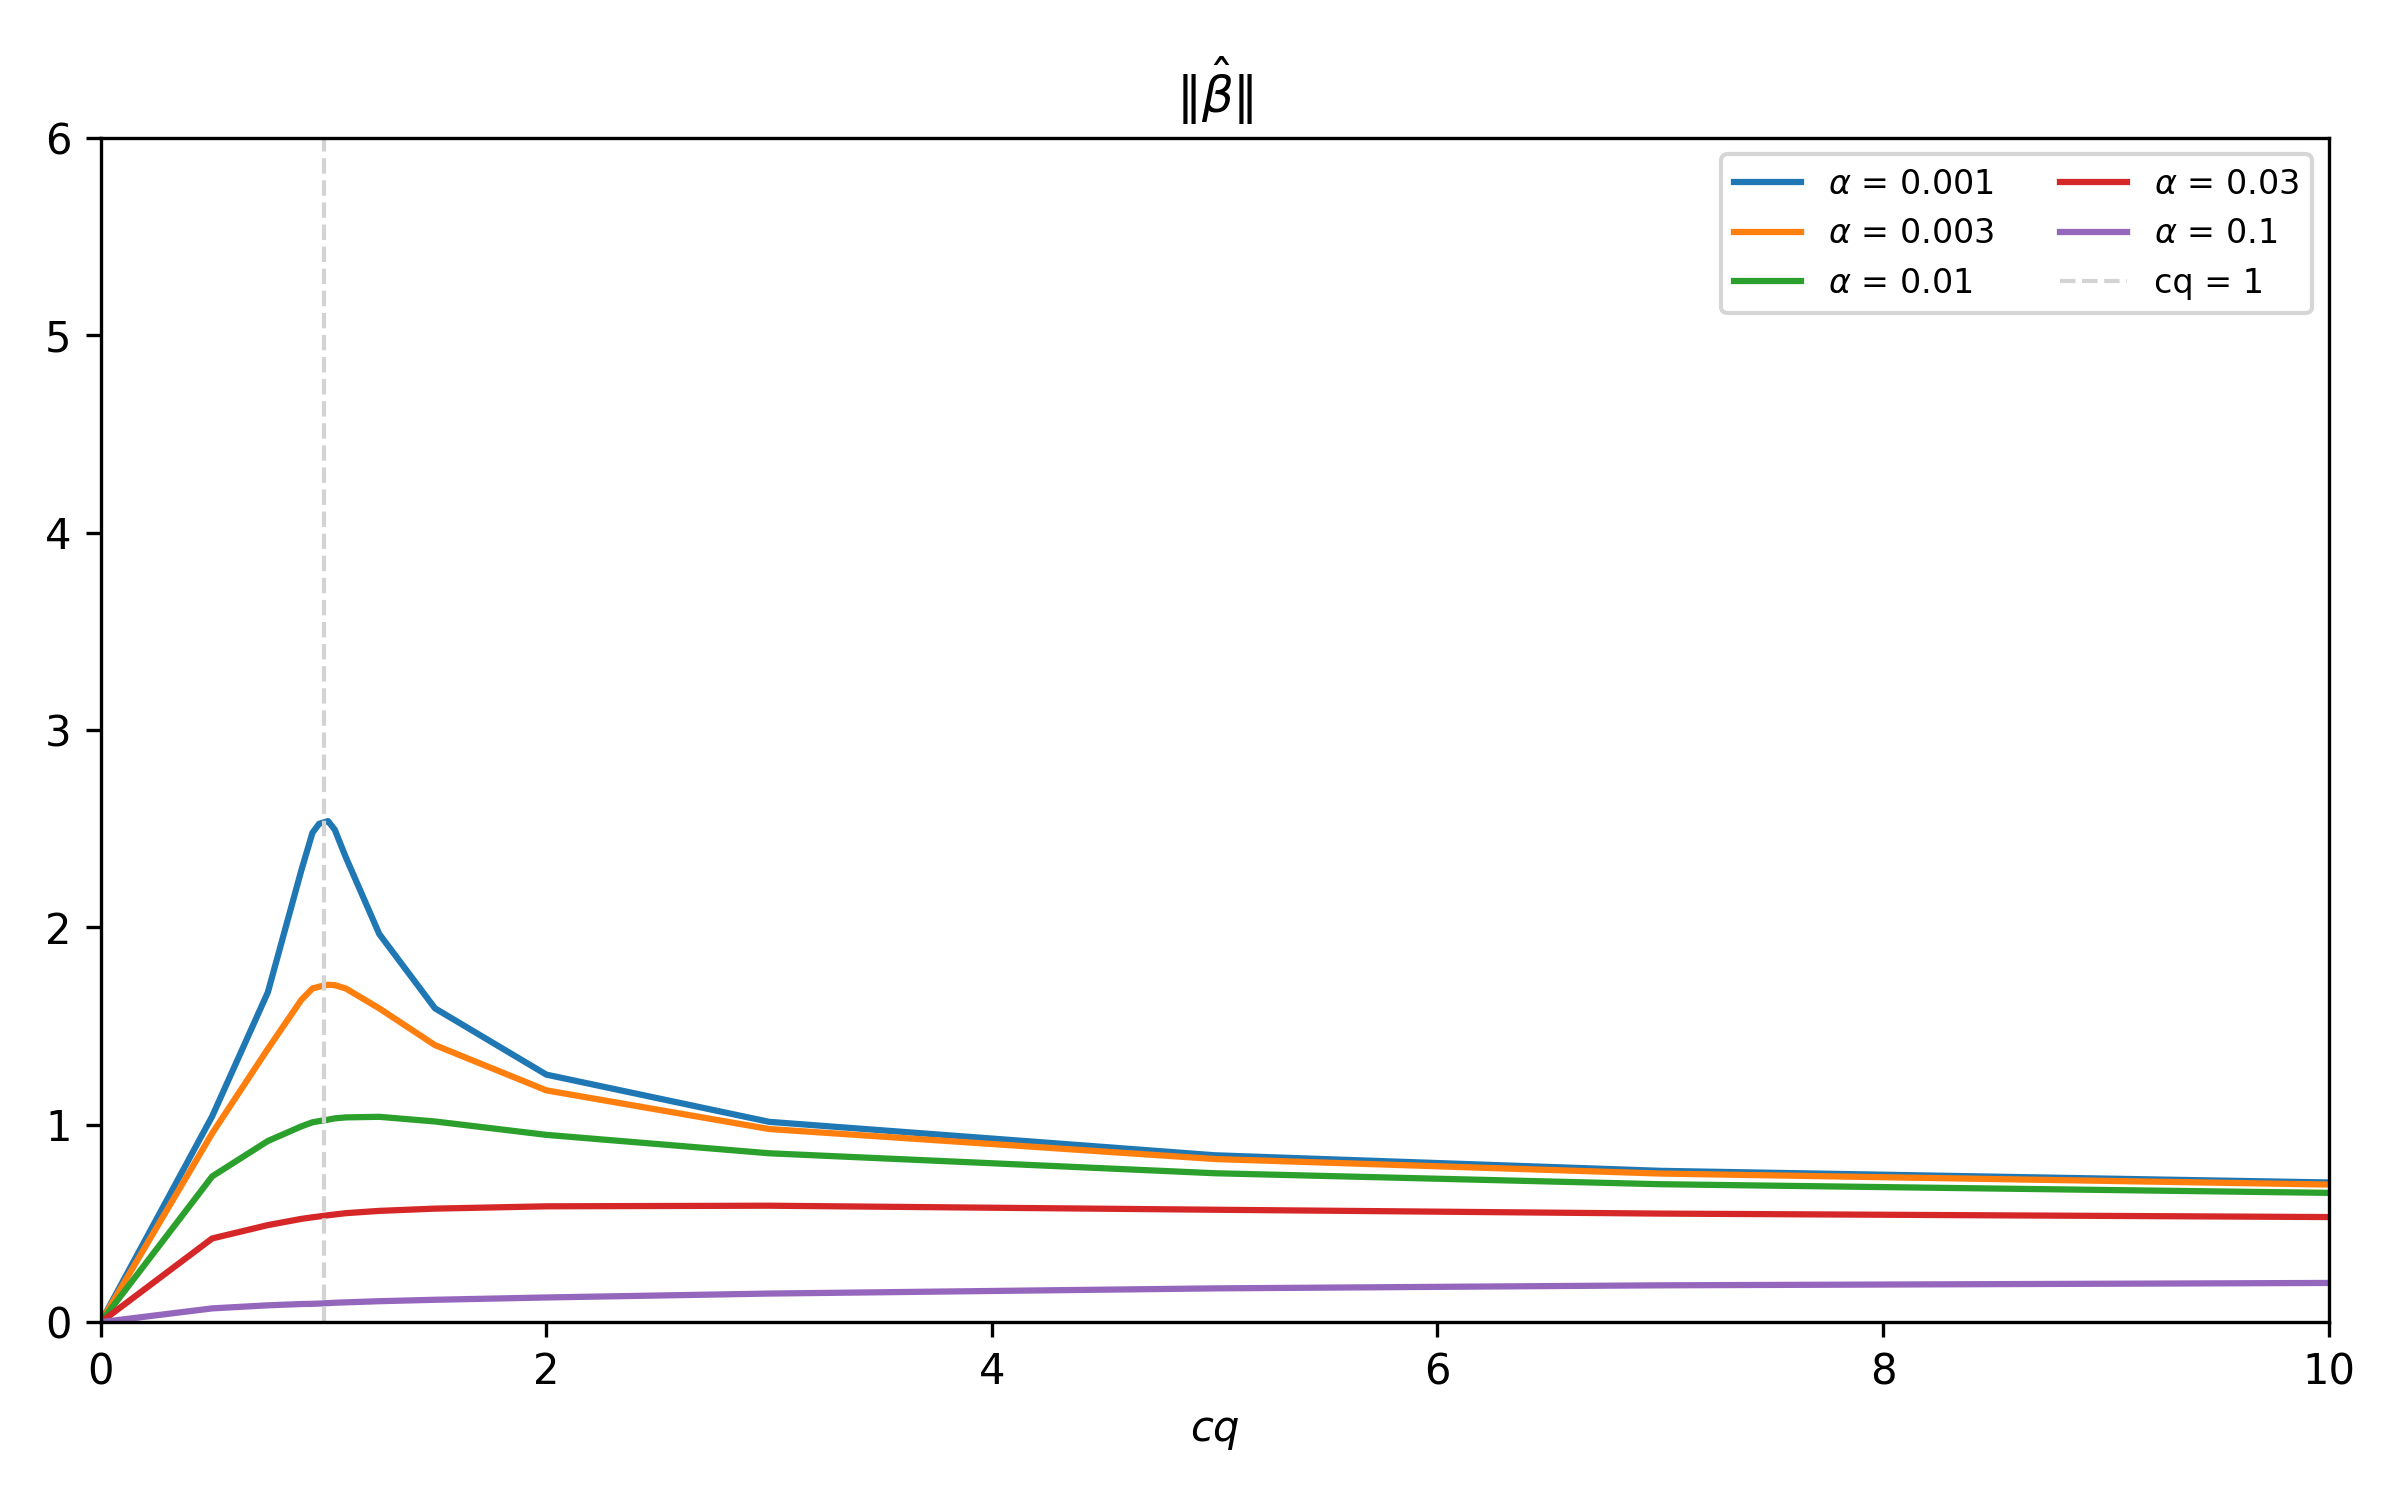
\includegraphics[width=\linewidth]{task1_2/task2_result_20261008_205656/beta_norm_vs_cq.png}
        \caption{Coefficient norm.}
    \end{subfigure}
    \caption{Out-of-sample Lasso results, averaged over 50 replications. The
    dashed line marks $cq=1$ and the displayed axes clip some interpolation
    extremes. The panels are produced by \texttt{plot\_lasso\_results()} in
    \texttt{task1\_2/plot\_results.py} from
    \texttt{task1\_2/task2\_result\_20261008\_205656/results.csv}.}
    \label{fig:task2-results}
\end{figure}

\clearpage
\section{Task 3: Predictions for Data Sets A, B, and C}

\subsection{Validation and model selection}

For each data set, the time index is excluded from the predictor matrix and
the last 20\% of the labeled observations are retained as a chronological
validation block. This gives 120 validation observations for A, 48 for B,
and 72 for C. Ridge, Lasso, and a one-hidden-layer neural network are fitted
on the preceding observations and evaluated using the same four criteria as
in Tasks~1 and 2. The primary selection criterion is fixed in advance as
$R^2_{\mathrm{paper}}$; expected timing return and the two Sharpe measures
are retained as economic diagnostics. Fixing one selection rule is important
because choosing a different model or parameter for whichever metric happens
to look strongest would add another layer of validation overfitting,
especially for B and C, whose holdout blocks are small.

The initial grids identify the relevant region for each estimator. The
selected model is then exploited in three successively narrower searches,
reported in Table~\ref{tab:task3-exploit}. Each round centers the next grid on
the preceding maximizer of $R^2_{\mathrm{paper}}$. The search is stopped after
the third round because the remaining differences are small relative to the
size of the validation blocks. After selection, the chosen specification is
refitted on all labeled observations and used to produce the hidden-data
predictions.

\begin{table}[htbp]
    \centering
    \small
    \caption{Task 3 hyperparameter exploitation rounds.}
    \label{tab:task3-exploit}
    \begin{tabular}{clllr}
        \toprule
        Data set & Model & Round & Search grid & Best parameter \\
        \midrule
        A & Ridge & 1 & $z\in[1.5,5.0]$ & $4.0$ \\
        A & Ridge & 2 & $z\in[3.4,4.6]$, step $0.2$ & $3.8$ \\
        A & Ridge & 3 & $z\in[3.65,3.95]$, step $0.05$ & $3.75$ \\
        \midrule
        B & Lasso & 1 & $\alpha\in[0.10,0.14]$, step $0.005$ & $0.120$ \\
        B & Lasso & 2 & $\alpha\in[0.116,0.124]$, step $0.002$ & $0.122$ \\
        B & Lasso & 3 & $\alpha\in[0.1200,0.1240]$, step $0.0005$ & $0.1215$ \\
        \midrule
        C & Lasso & 1 & $\alpha\in[0.15,0.21]$, step $0.01$ & $0.1900$ \\
        C & Lasso & 2 & $\alpha\in[0.1800,0.2000]$, step $0.0025$ & $0.1875$ \\
        C & Lasso & 3 & $\alpha\in[0.1850,0.1900]$, step $0.0005$ & $0.1865$ \\
        \bottomrule
    \end{tabular}
\end{table}

\paragraph{Data set A.}
Data set A has 600 observations and 600 predictors. Ridge is the only
candidate model with positive validation $R^2_{\mathrm{paper}}$. The final
local search has a broad, nearly flat maximum over $z=3.7$--$3.9$, with the
largest value, $0.042628$, at $z=3.75$. This flatness supports selecting the
interior value rather than extending the search to an unnecessarily precise
decimal. The corresponding timing return and paper Sharpe are $0.056045$ and
$0.171803$. In comparison, the best Lasso specification in the candidate
experiment has $R^2_{\mathrm{paper}}=-0.010871$ and negative timing and Sharpe
measures. The selected neural network has a positive timing return of
$0.144969$ but $R^2_{\mathrm{paper}}=-0.105352$, indicating that its output
scale is poorly calibrated despite some directional information. Ridge
therefore gives the best balance of prediction accuracy and economically
positive timing performance for A.

\pagebreak
\paragraph{Data set B.}
Data set B is strongly overparameterized, with 240 observations and 2400
predictors. Lasso is preferred because its coordinate-wise shrinkage can
discard irrelevant predictors rather than retaining all 2400 directions.
The three exploitation rounds move the local maximizer from $0.120$ to
$0.122$ and finally to $\alpha=0.1215$. At this value,
$R^2_{\mathrm{paper}}=0.001634$, expected timing return is $0.059076$, and the
paper Sharpe is $0.199729$. The nearby value $\alpha=0.120$ has marginally
higher timing and Sharpe measures but marginally lower
$R^2_{\mathrm{paper}}$; $0.1215$ is retained to preserve the pre-specified
selection rule. Ridge produces $R^2_{\mathrm{paper}}=-0.061635$ together with
negative timing and Sharpe measures, while the selected neural network gives
$R^2_{\mathrm{paper}}=-0.465629$. Thus the choice of Lasso is not based only
on a fine difference inside its local grid: it also dominates the alternative
model classes on validation prediction accuracy and both economic metrics.

\paragraph{Data set C.}
Data set C contains 360 observations and 1800 predictors, so sparsity is again
more plausible than a dense unrestricted fit. The first Lasso experiment used
$\alpha=0.15$ and produced $R^2_{\mathrm{paper}}=-0.001020$; a much stronger
penalty, $\alpha=0.30$, eliminated every coefficient and reduced the model to
the zero-prediction benchmark. Expanding and then narrowing the non-degenerate
region yields $\alpha=0.1865$, where $R^2_{\mathrm{paper}}=0.004597$ and all
three economic metrics are positive. By contrast, the best Ridge candidate
has $R^2_{\mathrm{paper}}=-0.073618$ and negative timing performance, and the
selected neural network has $R^2_{\mathrm{paper}}=-0.724517$. The final Lasso
penalty therefore represents the interior compromise between the noisy,
weakly penalized solutions and the all-zero solution generated by excessive
shrinkage.

\subsection{Final models and prediction files}

Table~\ref{tab:task3-validation} records the specifications selected under
the common validation rule. The reported prediction files are generated only
after refitting these specifications on the full labeled samples; their row
counts agree with the corresponding hidden feature files, as shown in
Table~\ref{tab:task3-predictions}.

\begin{table}[htbp]
    \centering
    \small
    \caption{Task 3 final validation results selected by
    $R^2_{\mathrm{paper}}$.}
    \label{tab:task3-validation}
    \begin{tabular}{clrrrrr}
        \toprule
        Data set & Model and parameter & $R^2_{\mathrm{paper}}$
        & $\mathbb E[R^\pi]$ & SR$_{\mathrm{paper}}$
        & SR$_{\mathrm{variance}}$ & $\|\widehat\beta\|_2$ \\
        \midrule
        A & Ridge, $z=3.75$
        & $0.042628$ & $0.056045$ & $0.171803$ & $0.174396$ & $0.233292$ \\
        B & Lasso, $\alpha=0.1215$
        & $0.001634$ & $0.059076$ & $0.199729$ & $0.203836$ & $0.320890$ \\
        C & Lasso, $\alpha=0.1865$
        & $0.004597$ & $0.003104$ & $0.091762$ & $0.092151$ & $0.037342$ \\
        \bottomrule
    \end{tabular}
\end{table}

\begin{table}[htbp]
    \centering
    \small
    \caption{Task 3 final prediction files.}
    \label{tab:task3-predictions}
    \begin{tabular}{clp{0.62\textwidth}}
        \toprule
        Data set & Observations & Prediction file \\
        \midrule
        A & $1000$ &
        \path{task3/A_ridge_result_20261010_155038/predictions_A.csv} \\
        B & $4000$ &
        \path{task3/B_lasso_result_20261010_155133/predictions_B.csv} \\
        C & $2000$ &
        \path{task3/C_lasso_result_20261010_155221/predictions_C.csv} \\
        \bottomrule
    \end{tabular}
\end{table}

\section{Task 4: Generalization and Overfitting in Neural Networks}

\subsection{Main finding of Montanari and Urbani}

Montanari and Urbani~\cite{montanari2025} study gradient-based training of a
wide two-layer network,
\begin{equation}
    f(x;\theta)=\frac{1}{m}\sum_{j=1}^{m}a_j\sigma(w_j'x),
\end{equation}
on noisy data whose predictable component depends on a low-dimensional latent
projection. Their main discovery is a separation of learning time scales. With
small-complexity mean-field initialization, the network first learns the
latent feature: training and test errors fall together while the
generalization gap remains small. On a much longer time scale, the magnitude
of the second-layer weights grows, the training error continues toward zero,
and the network begins fitting sample-specific noise. The test error then
rises and the learned first-layer representation can move away from the true
latent direction, a phenomenon the authors call \emph{feature unlearning}.

This mechanism connects feature learning and lazy or kernel-like training in
one trajectory. Early stopping is therefore not merely a generic penalty on
the number of updates. It selects the earlier low-complexity representation
before the network reaches the high-complexity interpolation regime. The
paper further predicts that, at fixed sample ratio $\alpha=n/(md)$, the onset
of overfitting is delayed as width $m$ increases. This statement is distinct
from increasing width at a fixed data set, because holding $\alpha$ constant
also increases $n$.

\subsection{Finite-sample experiment}

I test the mechanism in a synthetic return-prediction problem. Characteristics
$x_t\in\mathbb R^{20}$ are standard Gaussian and the next-period return is
\begin{equation}
    R_{t+1}=\sigma(u'x_t)+\varepsilon_{t+1},
    \qquad \varepsilon_{t+1}\sim\mathcal N(0,\tau^2),
\end{equation}
where $u$ is a randomly drawn unit vector and
\begin{equation}
    \sigma(z)=\sqrt{0.9}z+\frac{z^3-3z}{6}.
\end{equation}
This is the single-index design used in the paper's Figure~4 and implies
$h(q)=0.9q+q^3/6$. The student network has $m=32$ hidden units. Setting
$\alpha=n/(md)=0.3$ gives $n=192$ training observations; independent
validation and test sets contain $2000$ and $5000$ observations. The noise
grid is $\tau\in\{0,0.1,0.2,0.3,0.4,0.5\}$, with five replications at each
level.

First-layer weights are initialized as normalized Gaussian vectors and are
projected back to the unit sphere after every update; all second-layer weights
start at $a_j=1$. I use SGD for $10{,}000$ updates with batch size $100$,
learning rate $0.1$, and no explicit regularization. The DGP and activation
are implemented by \texttt{generate\_data()} and \texttt{activation()} in
\path{task4/generate_data.py}; the update equations and checkpoint loop are in
\path{task4/task4.py}. At each checkpoint I record train, validation, and test
half-MSE, the complexity proxy
\begin{equation}
    C(t)=\frac{1}{m}\sum_{j=1}^m |a_j(t)|,
\end{equation}
and signal alignment
\begin{equation}
    A(t)=\operatorname{Corr}^2\!\left(
        f(X_{\mathrm{te}};\theta_t),\sigma(X_{\mathrm{te}}u)
    \right).
\end{equation}
The latter measures retention of the true predictable component rather than
alignment with noisy realized returns. Metrics and figures are produced by
\path{task4/test_metrics.py} and \path{task4/plot_results.py}.

\subsection{Results}

Figure~\ref{fig:task4-dynamics} shows a noise-dependent separation between
feature learning and overfitting. During the first few hundred updates,
training and test errors decline together and signal alignment rises from
approximately zero to above $0.9$. With $\tau=0$ or $0.1$, test error continues
to improve through update $10{,}000$. From $\tau=0.2$ onward, it instead has a
U-shape, and the minimizing checkpoint occurs progressively earlier as noise
increases. Table~\ref{tab:task4-results} quantifies this pattern.

At the paper's $\tau=0.3$, average test half-MSE is minimized at update $2774$
and then rises by $10.1\%$ by update $10{,}000$. Meanwhile, final training
half-MSE is $0.0168$, well below the unpredictable-noise benchmark
$\tau^2/2=0.045$. The network must therefore be fitting part of the realized
training noise rather than only learning the population signal. Over the same
late interval, complexity reaches $1.598$ and signal alignment falls from its
peak of $0.946$ to $0.929$. At $\tau=0.5$, the test-error increase is $13.4\%$,
complexity reaches $2.063$, and alignment declines to $0.863$. The noiseless
control has no test-error reversal and ends with alignment $0.982$. Together,
these comparisons give finite-sample evidence consistent with the paper's
mechanism: more label noise moves the useful stopping point earlier and makes
late complexity growth and feature unlearning more pronounced.

\begin{figure}[htbp]
    \centering
    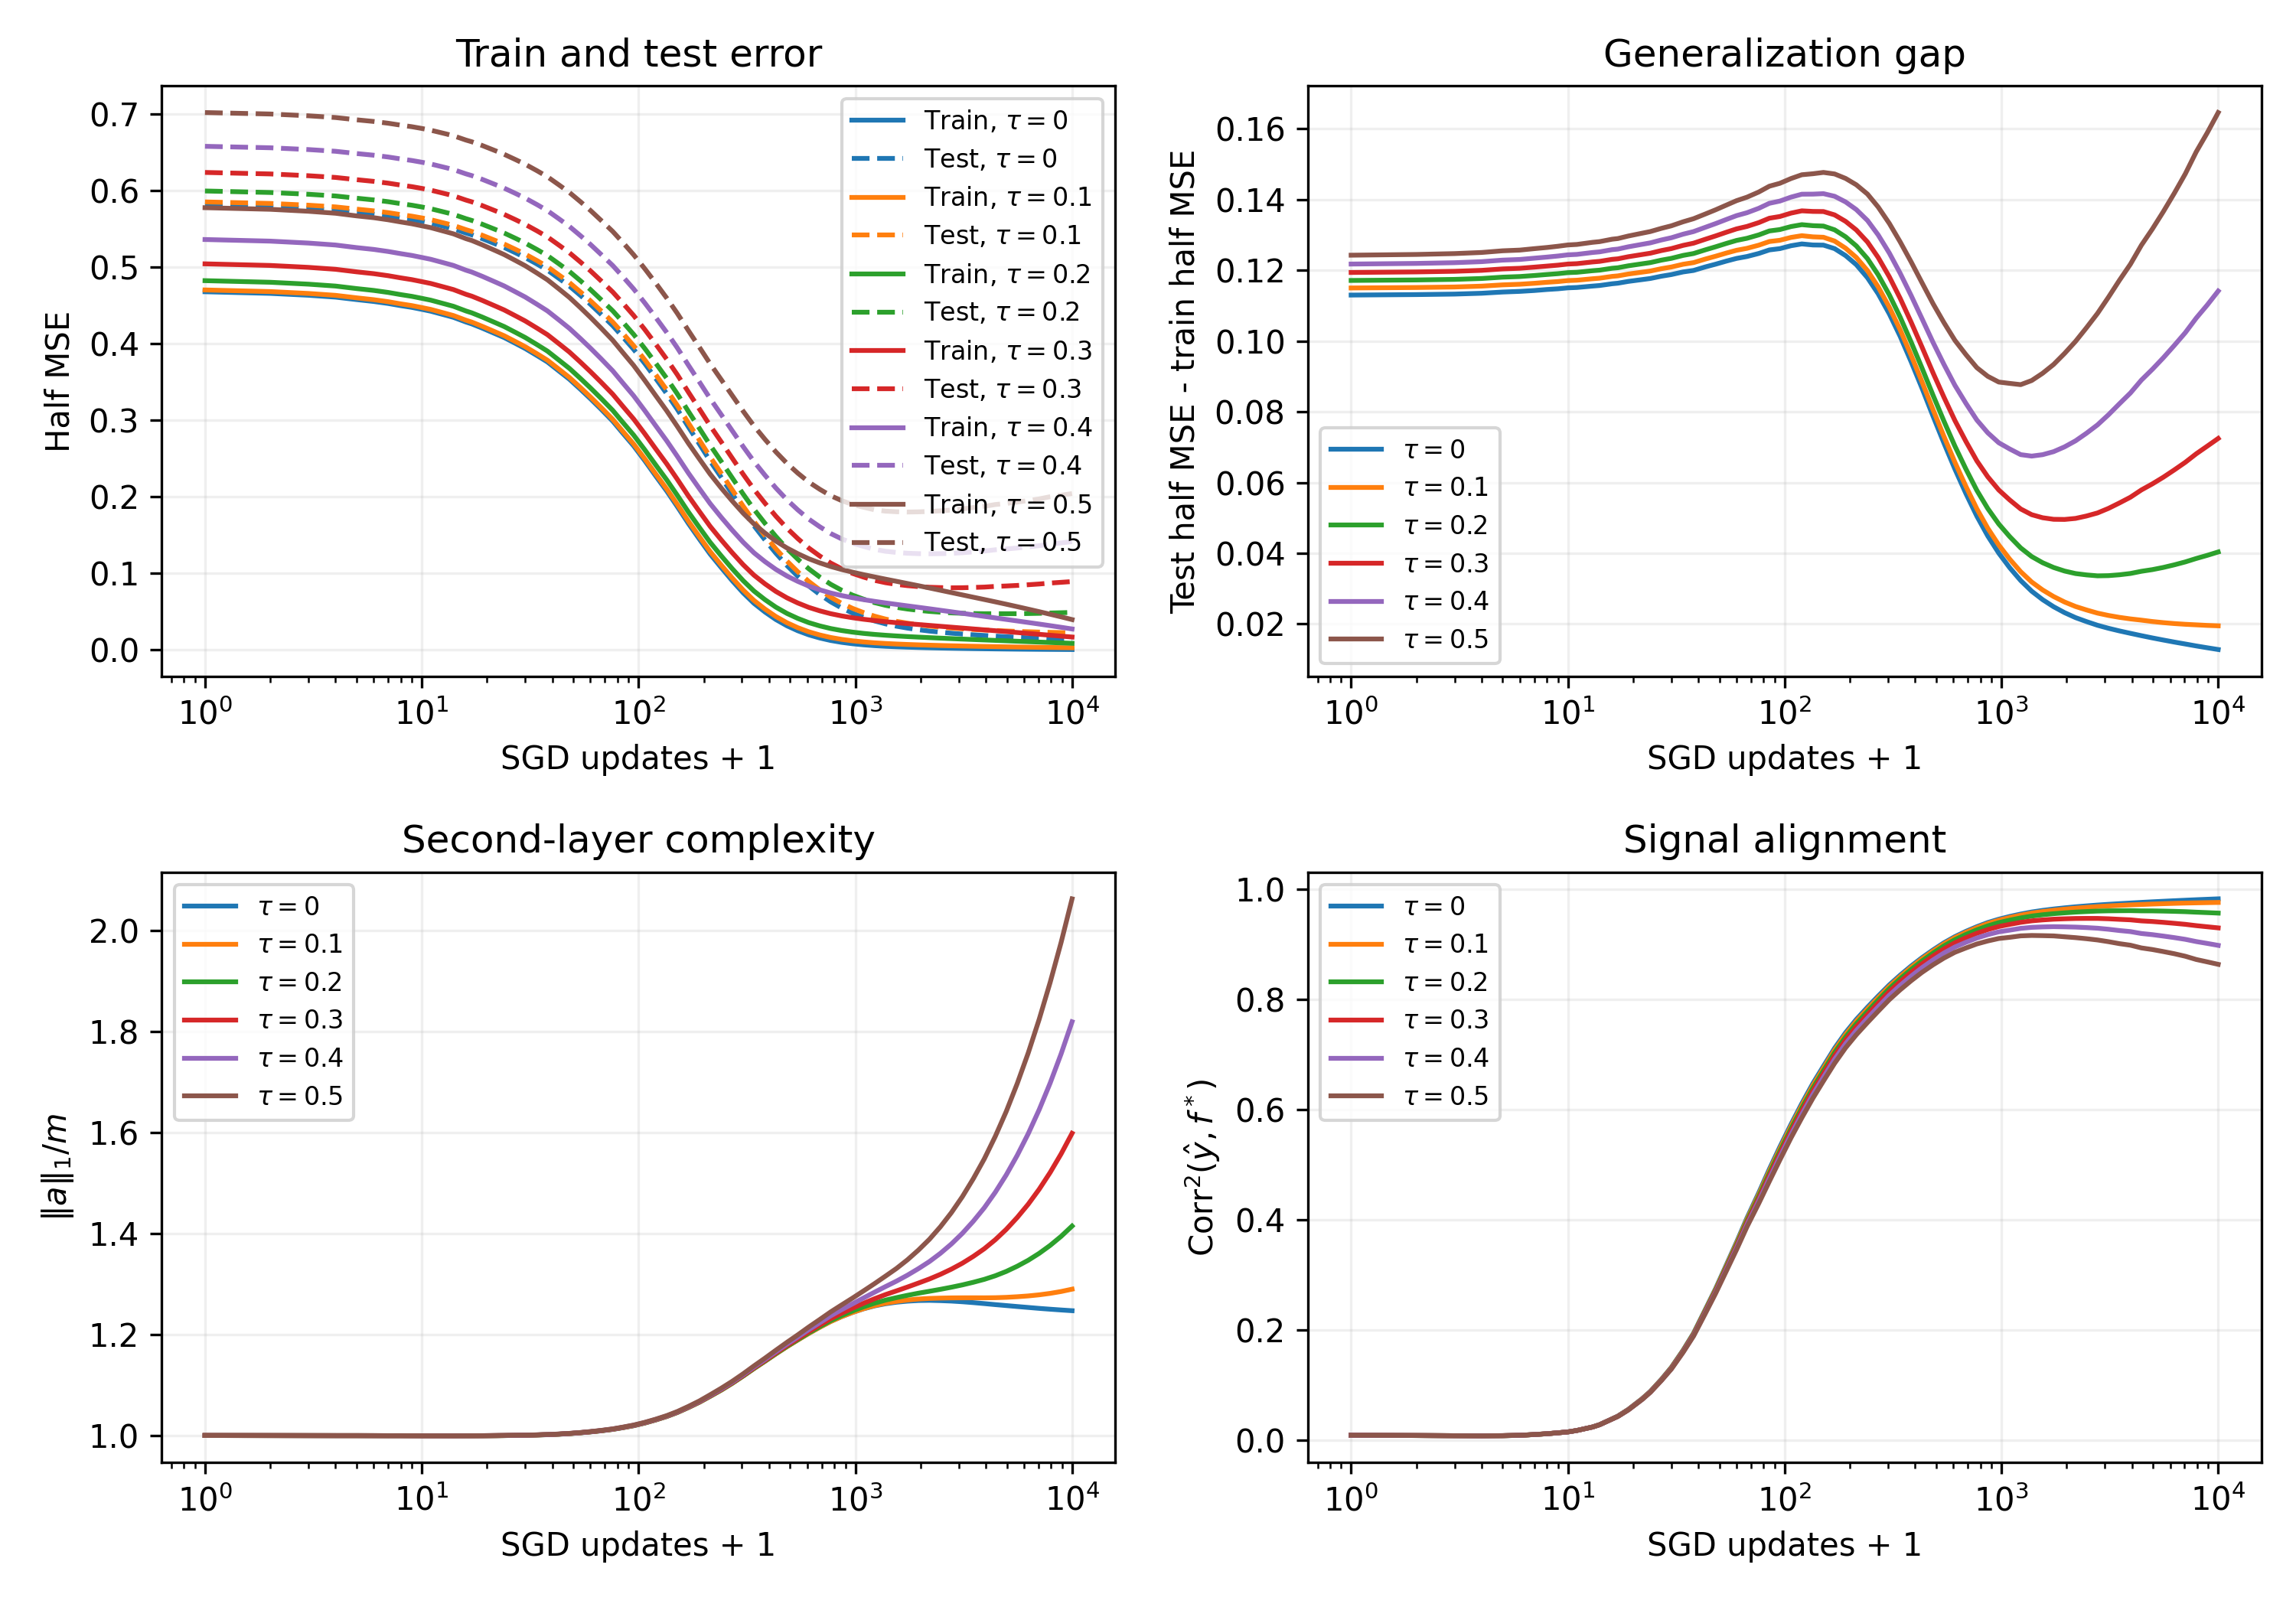
\includegraphics[width=\textwidth]{task4/task4_result_20261010_192233/training_dynamics.png}
    \caption{Training dynamics averaged over five replications. Solid and
    dashed curves in the upper-left panel are training and test half-MSE. The
    remaining panels report the generalization gap, second-layer complexity,
    and alignment with the noiseless latent signal. The horizontal axis is
    shown on a log scale.}
    \label{fig:task4-dynamics}
\end{figure}

\clearpage
\begin{table}[htbp]
    \centering
    \small
    \caption{Noise, early stopping, and late-training outcomes. The test-error
    increase compares update $10{,}000$ with the minimum of the mean test
    curve.}
    \label{tab:task4-results}
    \begin{tabular}{rrrrrr}
        \toprule
        $\tau$ & Best update & Best test half-MSE & Increase & Final $C(t)$
        & Final $A(t)$ \\
        \midrule
        $0.0$ & $10000$ & $0.0133$ & $0.0\%$  & $1.247$ & $0.982$ \\
        $0.1$ & $10000$ & $0.0223$ & $0.0\%$  & $1.290$ & $0.975$ \\
        $0.2$ & $4968$  & $0.0473$ & $3.6\%$  & $1.415$ & $0.956$ \\
        $0.3$ & $2774$  & $0.0811$ & $10.1\%$ & $1.598$ & $0.929$ \\
        $0.4$ & $2197$  & $0.1255$ & $12.7\%$ & $1.819$ & $0.897$ \\
        $0.5$ & $1740$  & $0.1801$ & $13.4\%$ & $2.063$ & $0.863$ \\
        \bottomrule
    \end{tabular}
\end{table}

\subsection{Implication for financial machine learning}

The experiment interprets $u'x_t$ as a latent return factor and $\tau$ as the
strength of idiosyncratic return noise. Its practical implication is that a
falling in-sample loss is weak evidence that a return-prediction network is
still discovering tradable structure. In the noisy cases, training continues
to improve after out-of-sample accuracy has peaked, while the network becomes
more complex and less aligned with the population signal. A financial
workflow should therefore use a chronological validation block for early
stopping and should monitor prediction stability or weight growth alongside
training loss. The preferred checkpoint should be selected on validation
data; the test set in this experiment is used only for ex-post evaluation.

The evidence is deliberately qualitative. The network is much smaller than
the asymptotic model, the late-stage training error is small but not exactly
zero, and only one width is studied, so the experiment does not test the
paper's scaling law in $m$. The observed decline in alignment supports feature
unlearning but does not establish the full DMFT mechanism. Finally, the data
are i.i.d. Gaussian with one stable latent factor. Actual returns have weak
and changing signals, dependence, heavy tails, and trading costs, all of
which make validation design more difficult. These limitations strengthen,
rather than weaken, the practical case for conservative early stopping, but
they prevent interpreting the numerical thresholds as direct prescriptions
for a live strategy.

\section{Task 5: Video and Reproducibility}

% Add the video link and summarize clean-run commands and generated outputs.

\section{Conclusion}

% Summarize the main empirical and conceptual lessons across Tasks 1--4.

\begin{thebibliography}{9}

\bibitem{kelly2024}
Kelly, B. T., Malamud, S., and Zhou, K. (2024).
The virtue of complexity in return prediction.
\emph{Journal of Finance}, 79(1), 459--503.

\bibitem{montanari2025}
Montanari, A. and Urbani, P. (2025).
Dynamical decoupling of generalization and overfitting in large two-layer networks.
\emph{Advances in Neural Information Processing Systems}, 38.

\end{thebibliography}

\end{document}
